\begin{document}

\mode<presentation>{
\title{Spin Networks for Perfect Quantum State Transfer}
\author{dln-dev}
\date{February 22nd 2017}
%\logo{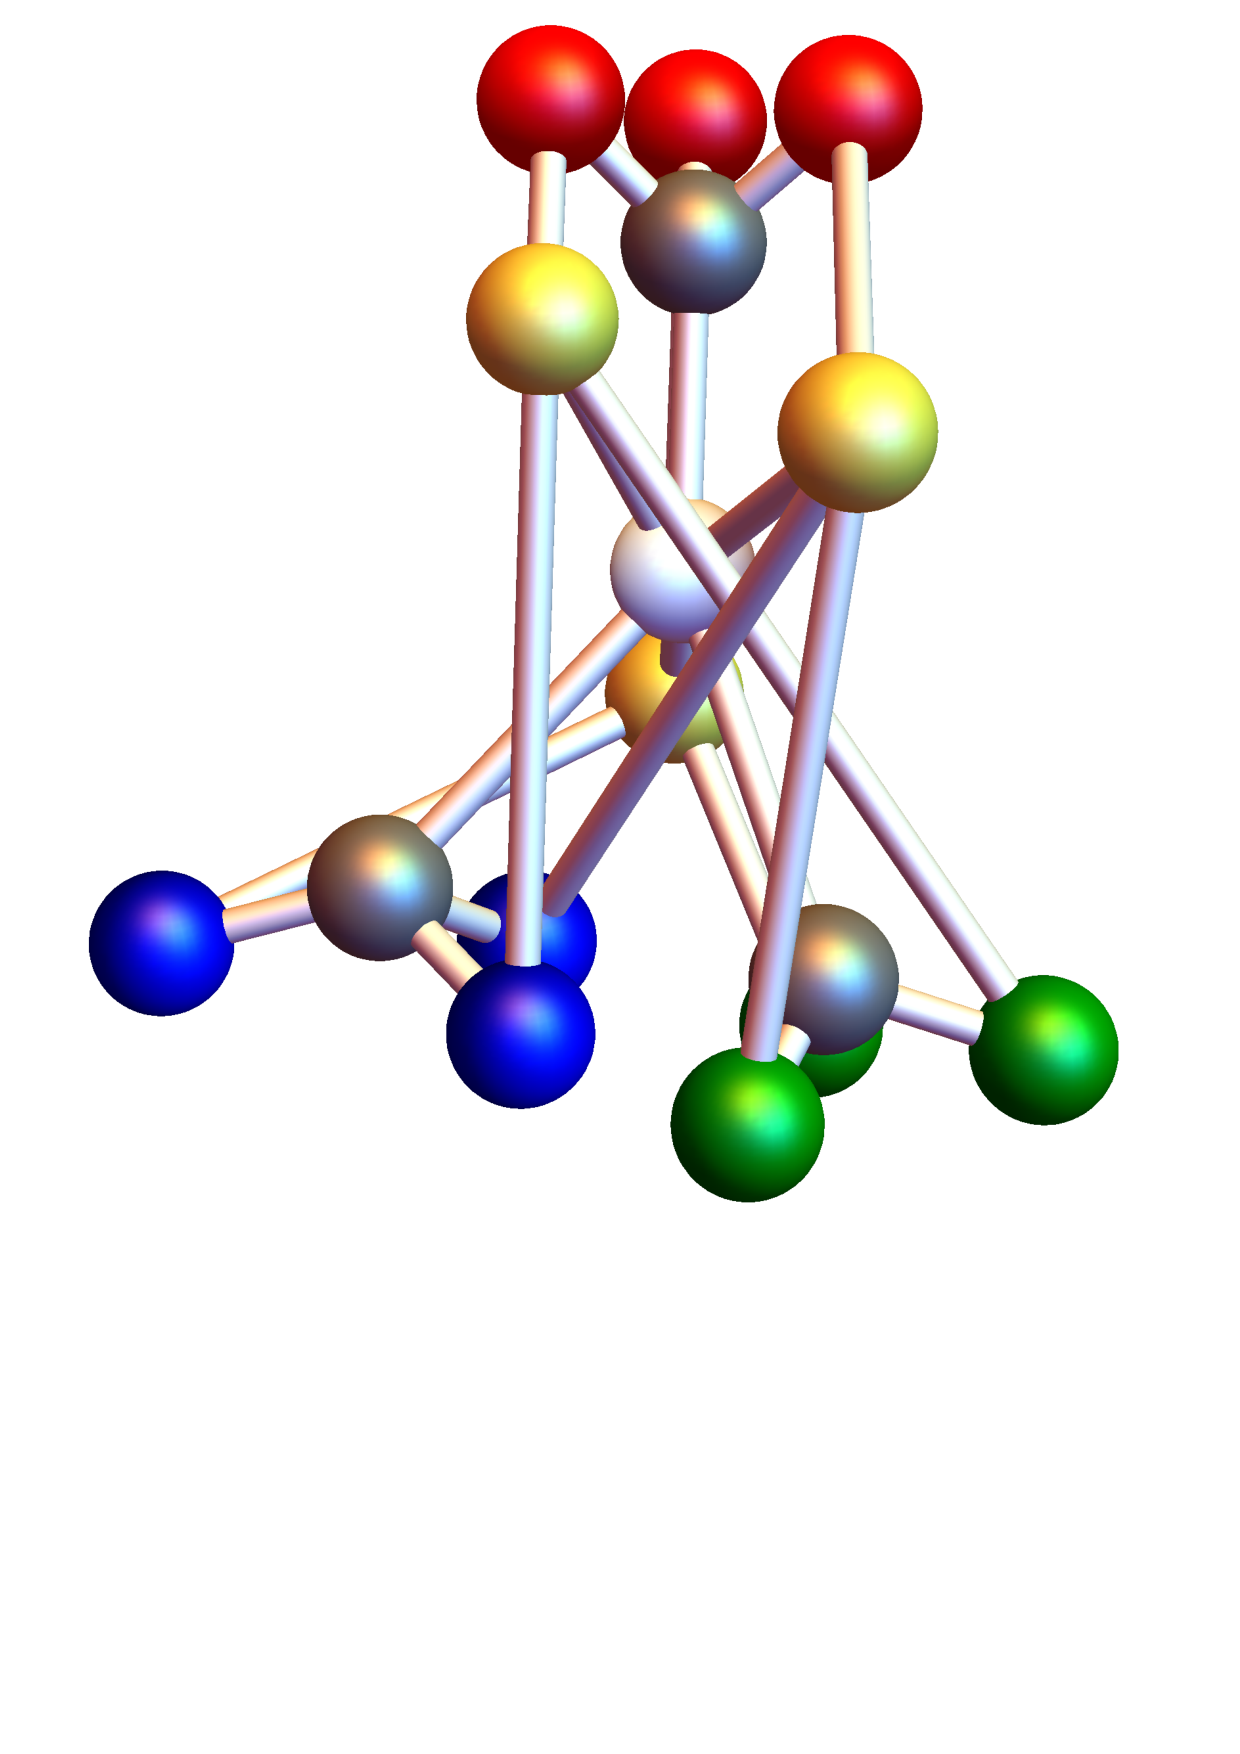
\includegraphics[width=\textwidth]{Images/switch_square}}
\titlegraphic{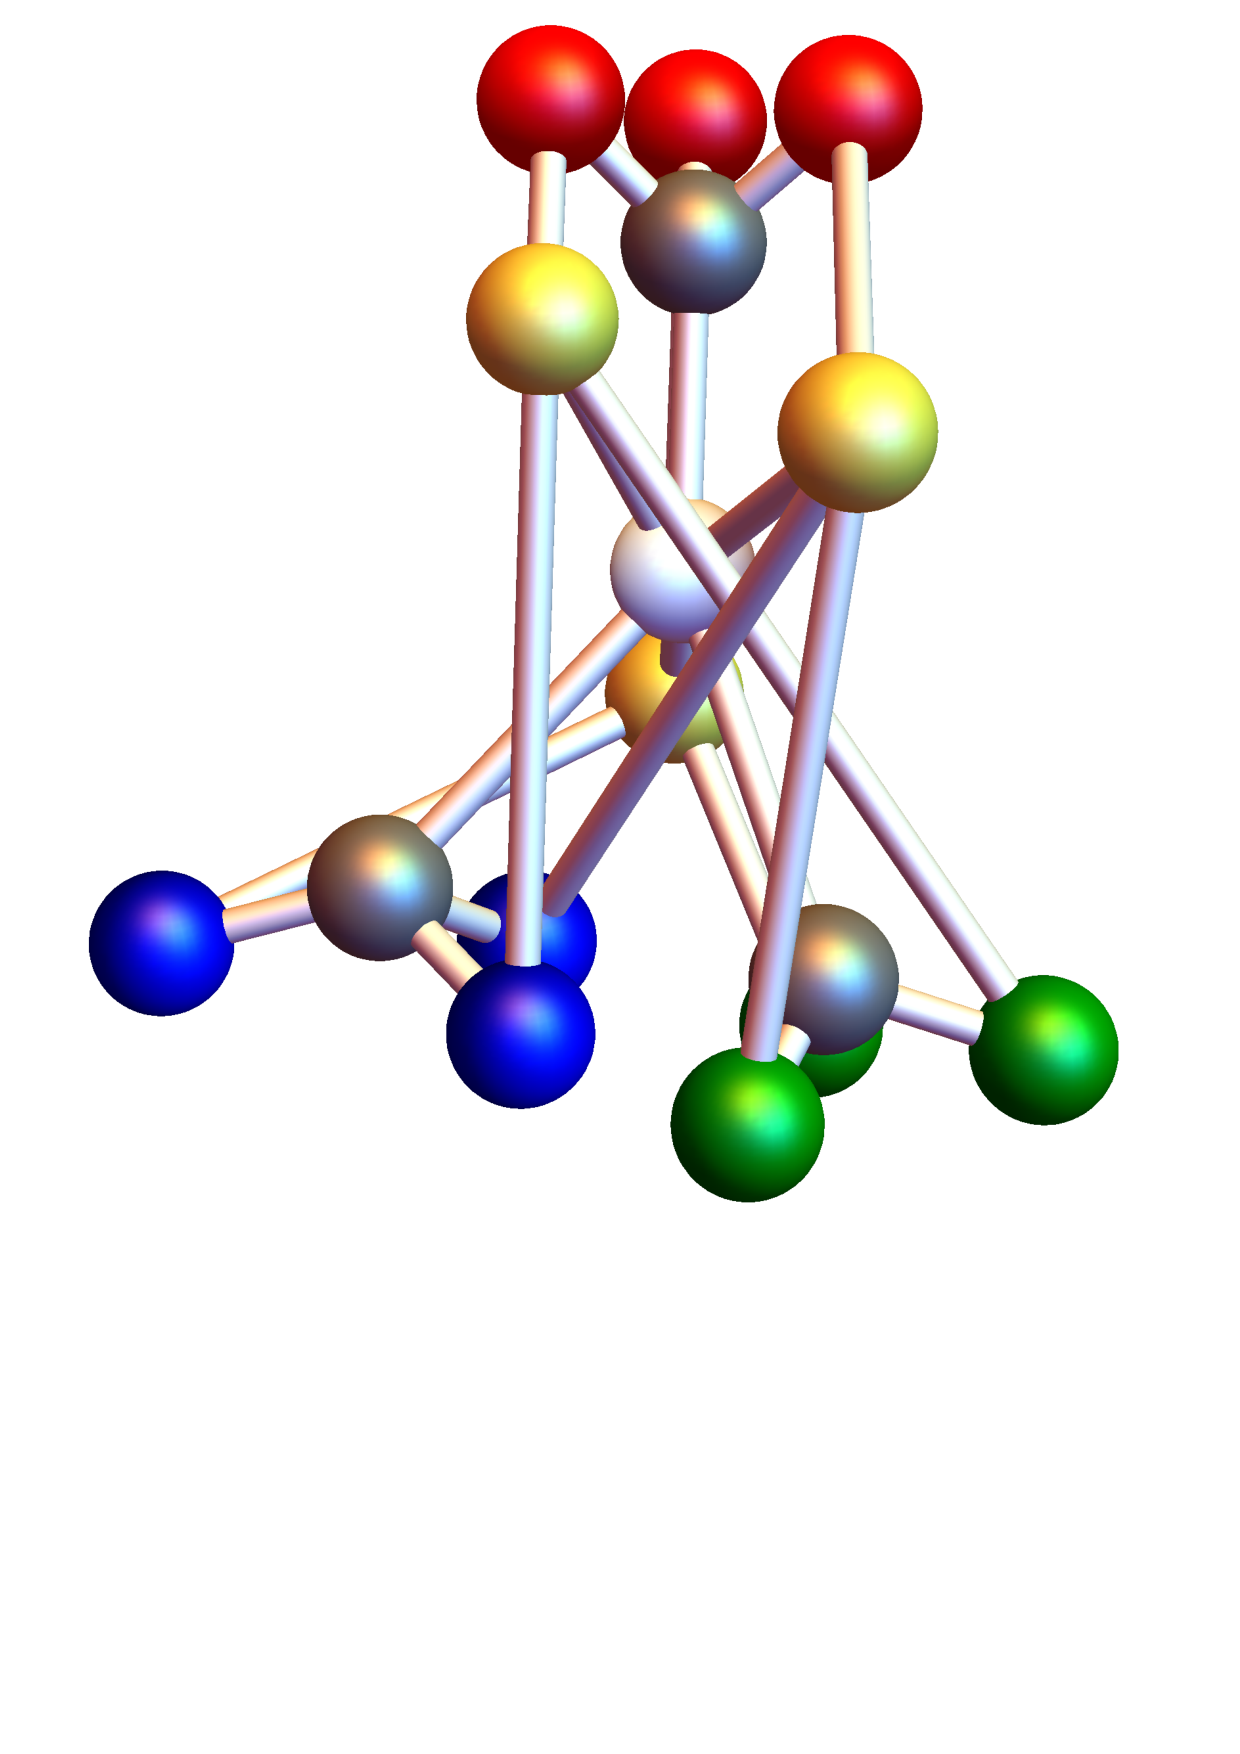
\includegraphics[width=0.1\textwidth]{Images/switch_square}}

\frame{\titlepage}
}

\mode<article>{\begin{titlepage}
	\center
	\vspace*{5.0cm}
	{ \huge \bfseries Spin Networks for Perfect Quantum State Transfer}\\[0.4cm]

	\textsc{\Large dln-dev}\\[1.5cm]
	{\large February 22nd 2017}\\[5.0cm]

	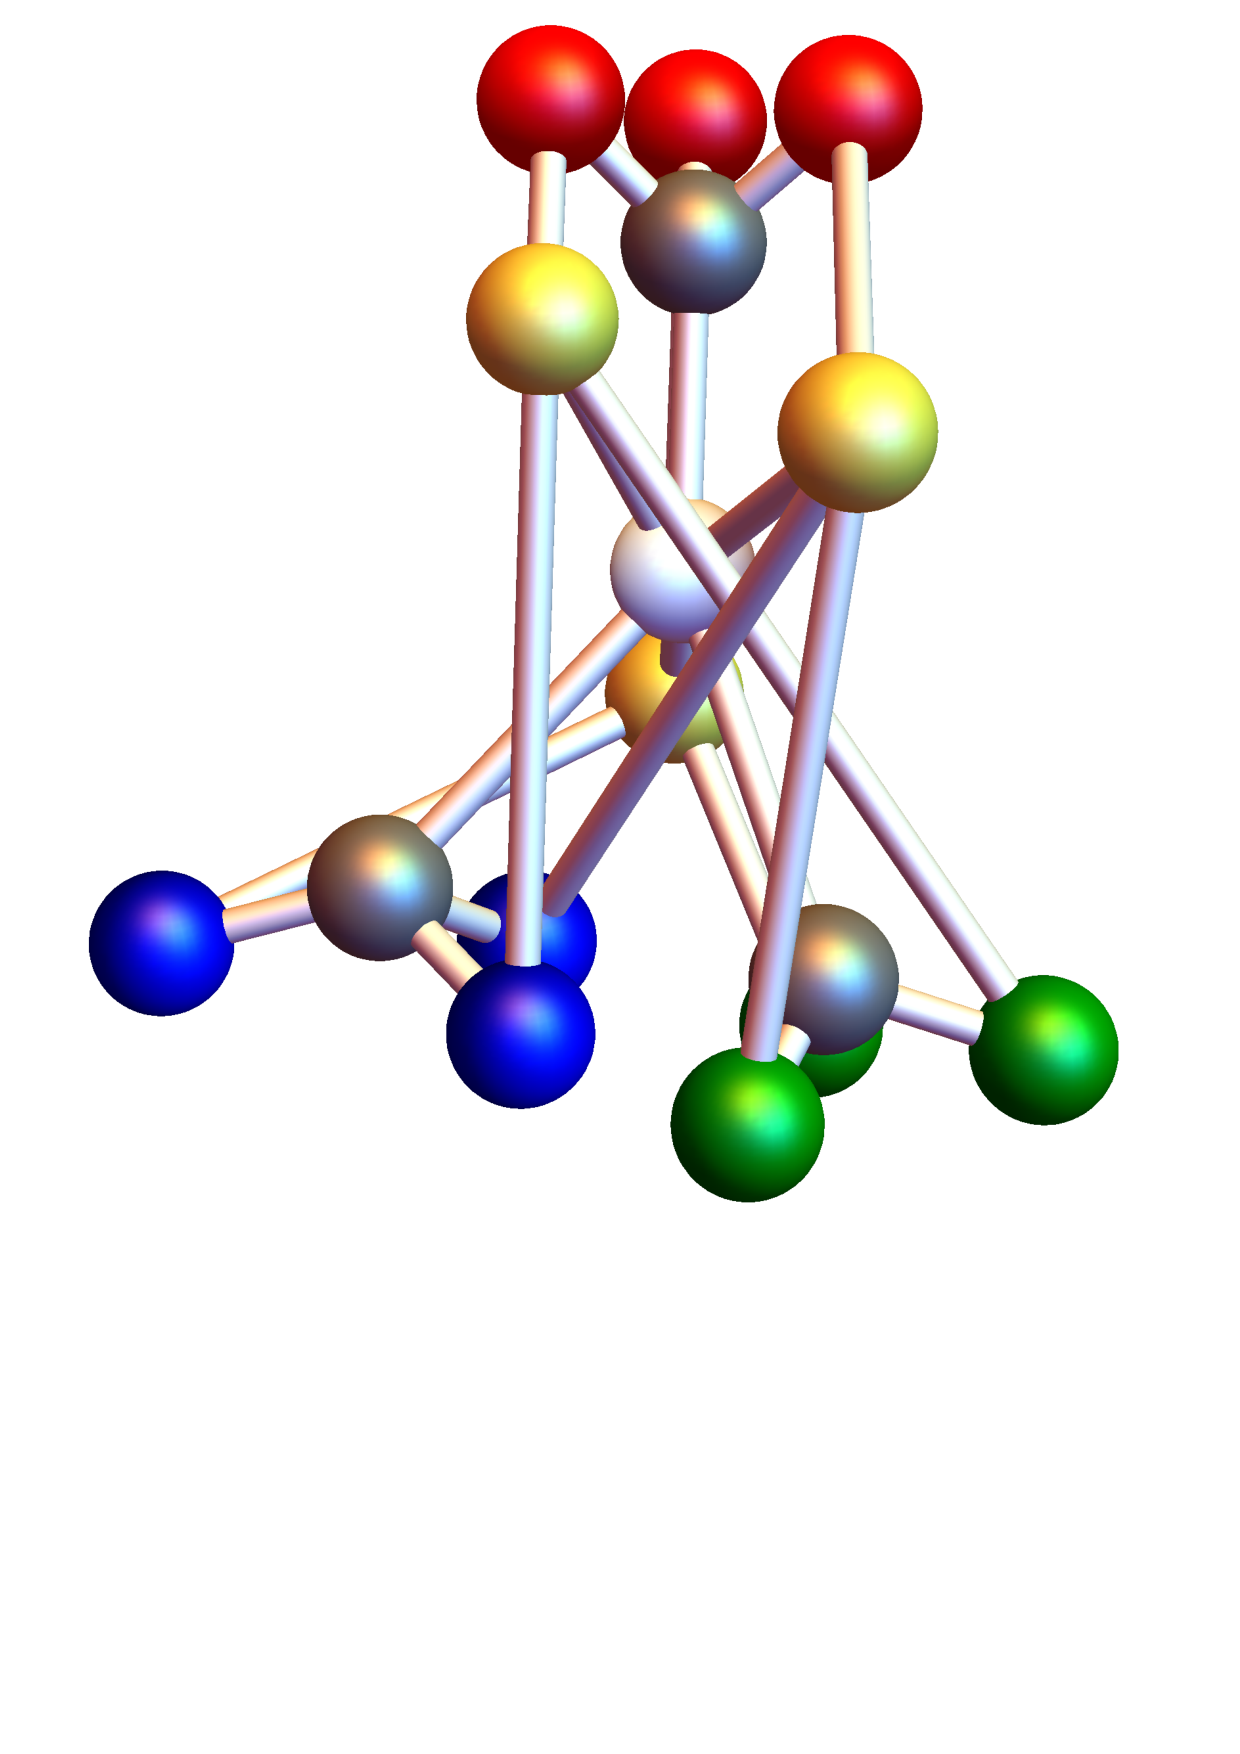
\includegraphics[width=0.3\textwidth]{Images/switch_square}\\[1cm]
	\vfill
\end{titlepage}

\tableofcontents}


\section{Model}

\subsection{Motivation}
\mode<presentation>{\begin{frame}{Spin Networks}\label{register}
	\begin{columns}[T]
		\begin{column}{0.5\textwidth}
			\centering
   			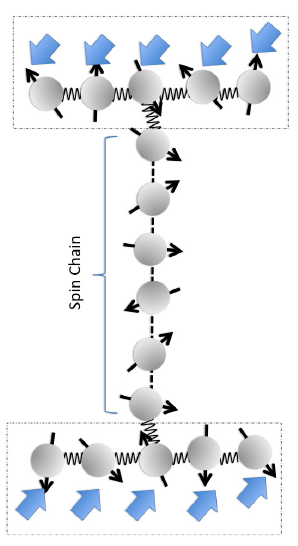
\includegraphics[width=0.7\textwidth]{Images/processor}
		\end{column}
		\begin{column}{0.5\textwidth}
			\centering
			\vspace*{2cm}
    		\begin{itemize}
    			\item Distributed design
    			\item Passive connections
    			\item Distance
    			\item Same material 
    		\end{itemize}
    		\vspace*{1cm}
    		$\rightarrow$ Spin networks!
		\end{column}
	\end{columns}
	\vspace*{0.6cm}
	\footnotesize\textcolor{tugreen}{$\blacktriangleright$}\,\,\cite{Bose2014}\normalsize
\end{frame}}

\begin{center}
	\includeslide{register}
\end{center}

\noindent text 

\subsection{Model}
\mode<presentation>{\begin{frame}{Model}\label{model}
		\centering
   		\begin{exampleblock}{}
			\setlength\abovedisplayskip{-8pt}
			\begin{center}
			\[H_{XX}=\frac{1}{2}J\sum_{i=1}^{N}{\left[\sigma_i^x\sigma_{i+1}^x + \sigma_i^y\sigma_{i+1}^y\right]}\]
			\end{center}
		\end{exampleblock}
		\vspace*{0.5cm}
		\begin{itemize}
   			\item Spin-$\frac{1}{2}$ systems as qubits
   			\item Coupled by $x$ and $y$ component
   			\item Information encoded on $z$ component
   		\end{itemize}   		
\end{frame}}

\begin{center}
	\includeslide{turing}
\end{center}

\noindent text

\subsection{Graphs and Adjacency Matrices}
\mode<presentation>{\begin{frame}{Graphs and Adjacency Matrices}\label{graphs}
	\begin{itemize}
		\item $G = (V,E)$
		\item Edges undirected $\rightarrow E \subseteq \{\{i,j\}\colon i,j \in V\}$
		\item Single edges only $\rightarrow \{i,j\}$ unique
	\end{itemize}
	\begin{columns}[T]
		\begin{column}{0.5\textwidth}
			\centering
			\vspace*{1.5cm}
   			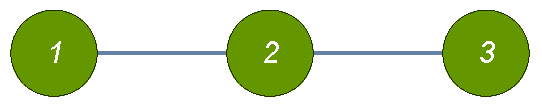
\includegraphics[width=0.85\textwidth]{Images/chain3-graph}
		\end{column}
		\begin{column}{0.5\textwidth}
			\centering
			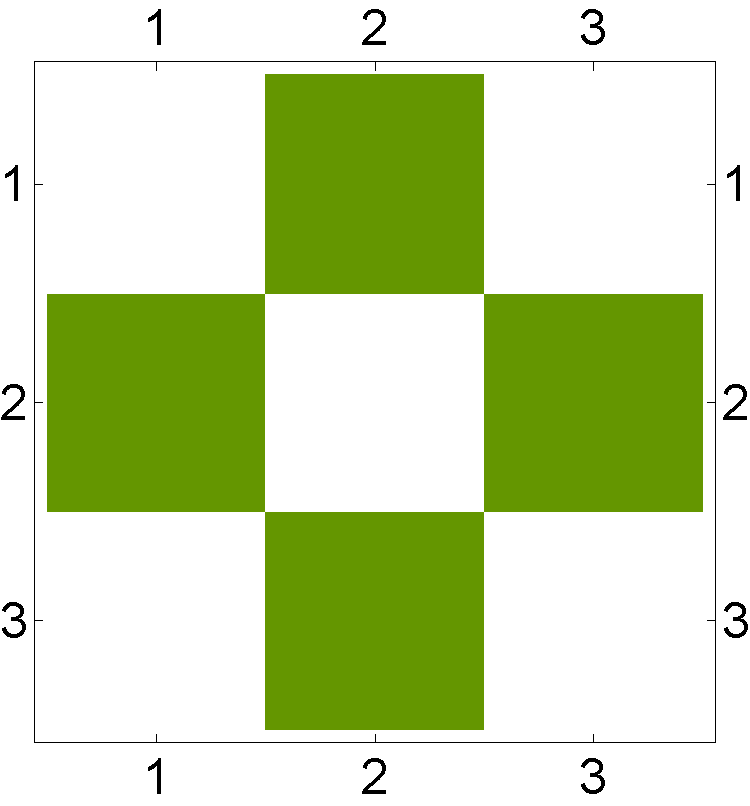
\includegraphics[width=0.7\textwidth]{Images/chain3-adjmat}
		\end{column}
	\end{columns}
\end{frame}}

\begin{center}
	\includeslide{complexity}
\end{center}

\noindent text


\mode<presentation>{\begin{frame}{Graphs and Adjacency Matrices}\label{graphs2}
	\begin{columns}[T]
		\begin{column}{0.5\textwidth}
			\centering
			\vspace*{0.5cm}
   			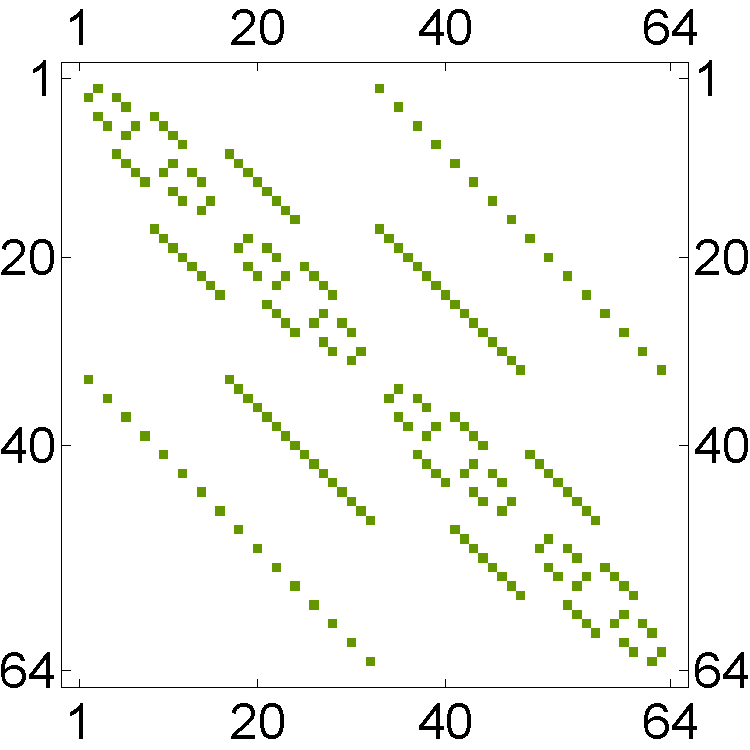
\includegraphics[width=0.85\textwidth]{Images/chain6p-fullhamiltonian} \\
		\begin{exampleblock}{}
			\setlength\abovedisplayskip{-8pt}
			\begin{center}
			\[ \left[H,\sigma_{tot}^z\right] = 0 \]
			\end{center}
		\end{exampleblock}
		\end{column}
		\begin{column}{0.5\textwidth}
			\centering
   			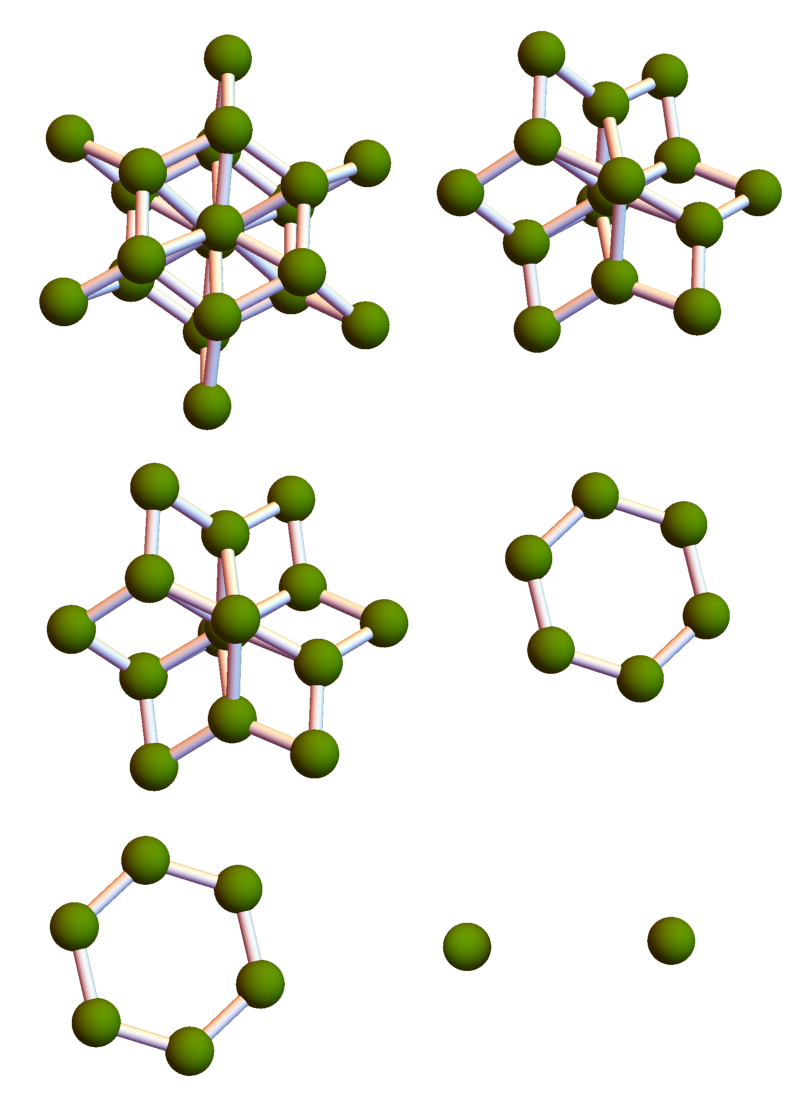
\includegraphics[width=0.85\textwidth]{Images/chain6p_fullgraph}
		\end{column}
	\end{columns}
\end{frame}}

\begin{center}
	\includeslide{complexity}
\end{center}

\noindent text


\mode<presentation>{\begin{frame}{Graphs and Adjacency Matrices}\label{graphs4}
	\begin{columns}[T]
		\begin{column}{0.5\textwidth}
			\centering
%			Restrict $H$ to single excitation
			\vspace*{0.5cm}
			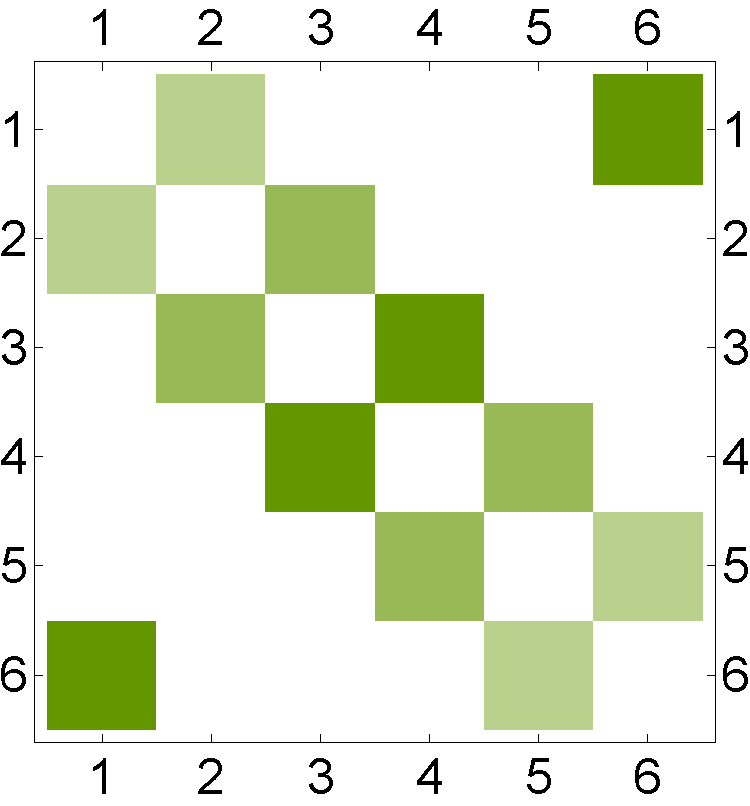
\includegraphics[width=0.9\textwidth]{Images/chain6vary-adjmat}	
		\end{column}
		\begin{column}{0.5\textwidth}
			\centering	
			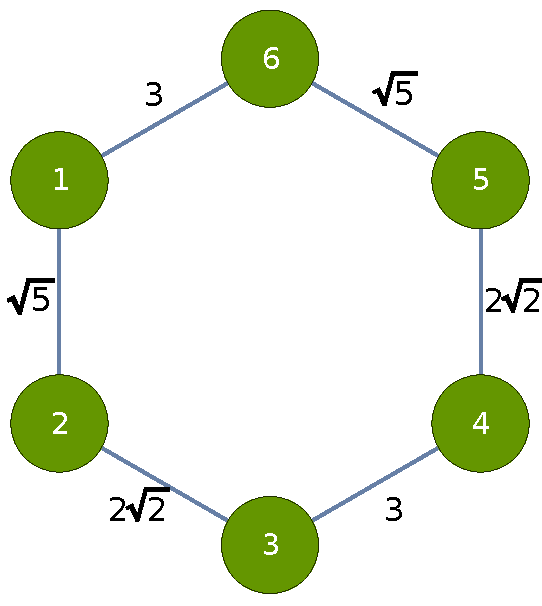
\includegraphics[width=\textwidth]{Images/chain6vary-graph}
		\end{column}
	\end{columns}
\end{frame}}

\begin{center}
	\includeslide{complexity}
\end{center}

\noindent text


\mode<presentation>{\begin{frame}{Cartesian Graph Product}\label{graphproduct}
	\begin{exampleblock}{}
	\setlength\abovedisplayskip{-8pt}
	\begin{center}
		$A_{G\times H} = A_G \otimes \text{1}_{\left|V_H\right|} + \text{1}_{\left|V_G\right|} \otimes A_H$
	\end{center}
	\end{exampleblock}
	\begin{columns}[T]
		\begin{column}{0.33\textwidth}
			\centering
   			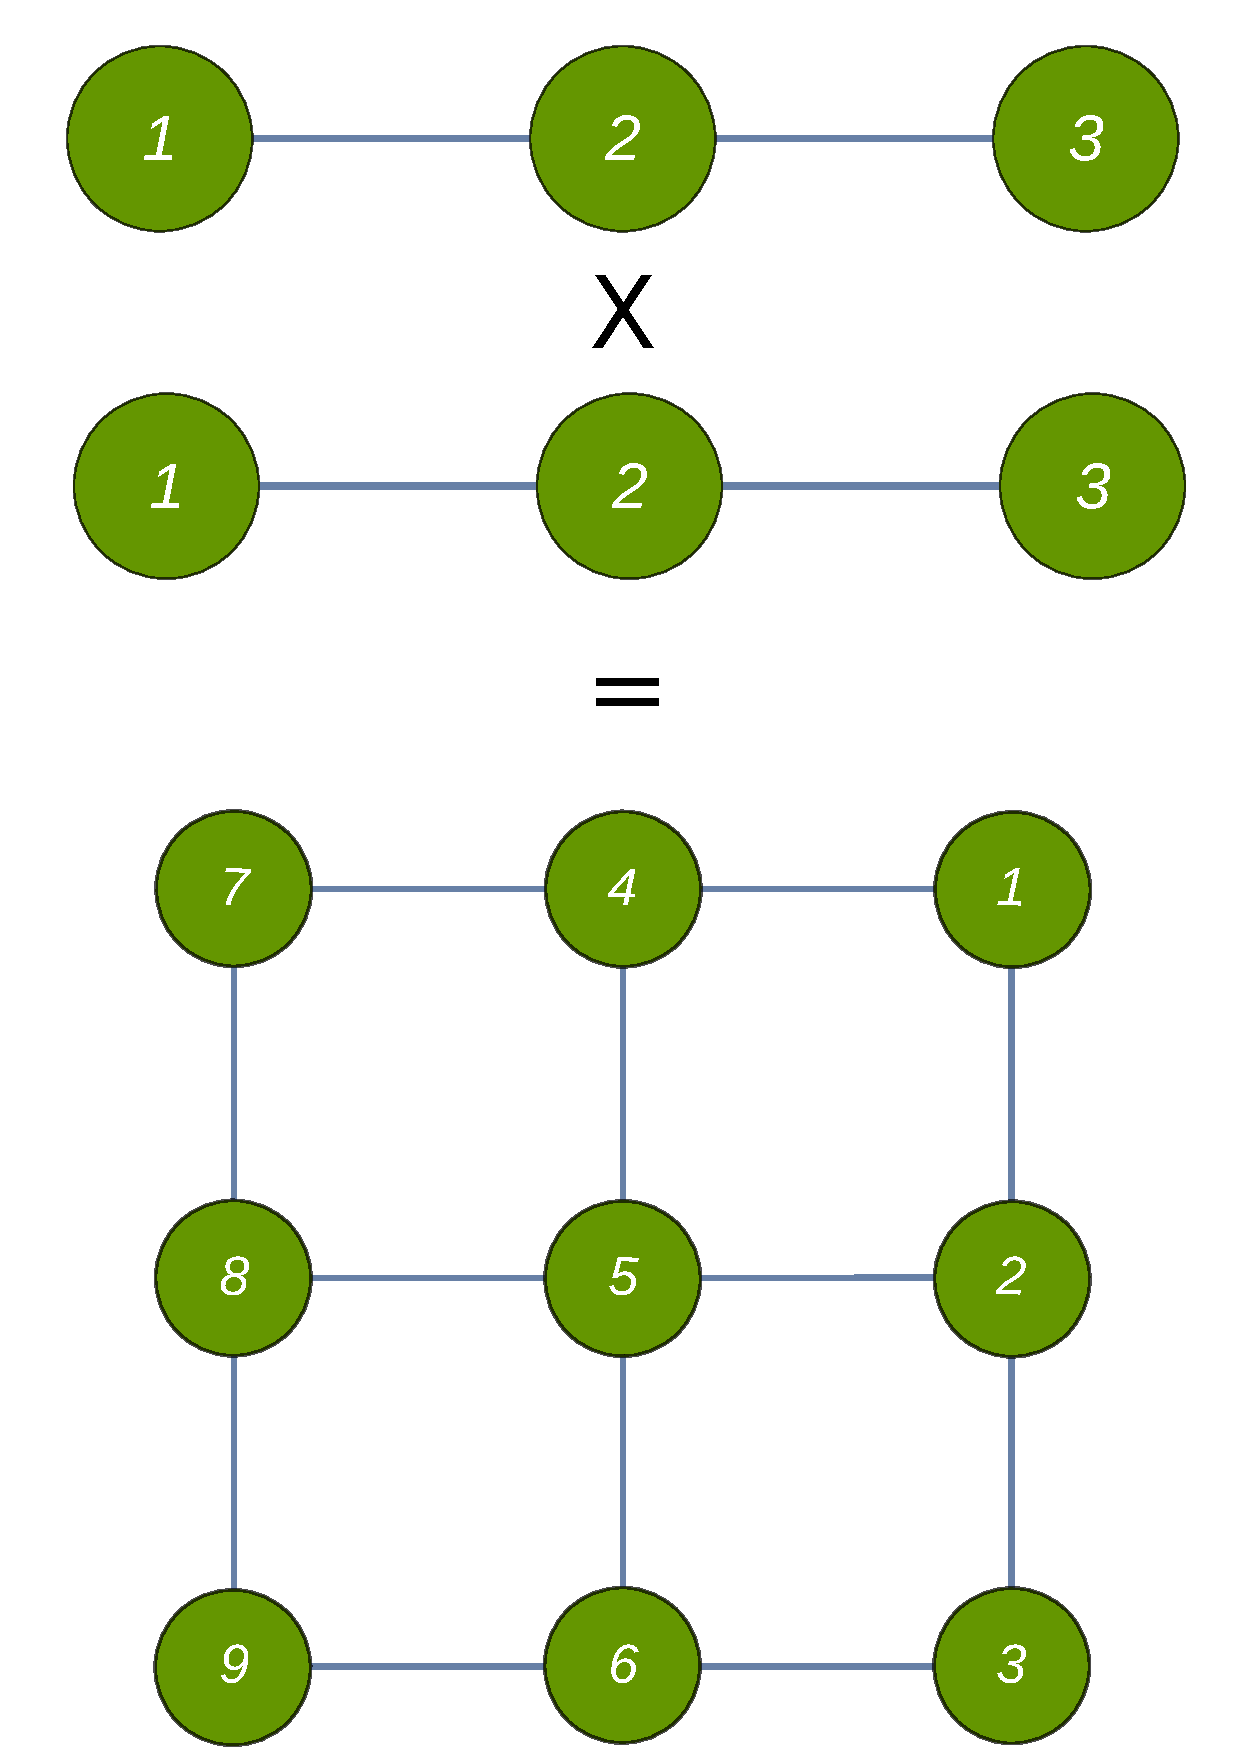
\includegraphics[trim=0mm 0 0 0mm, width=1.0\textwidth]{Images/graphprod_chain3_square} \\
		\end{column}
		\begin{column}{0.33\textwidth}
			\centering
   			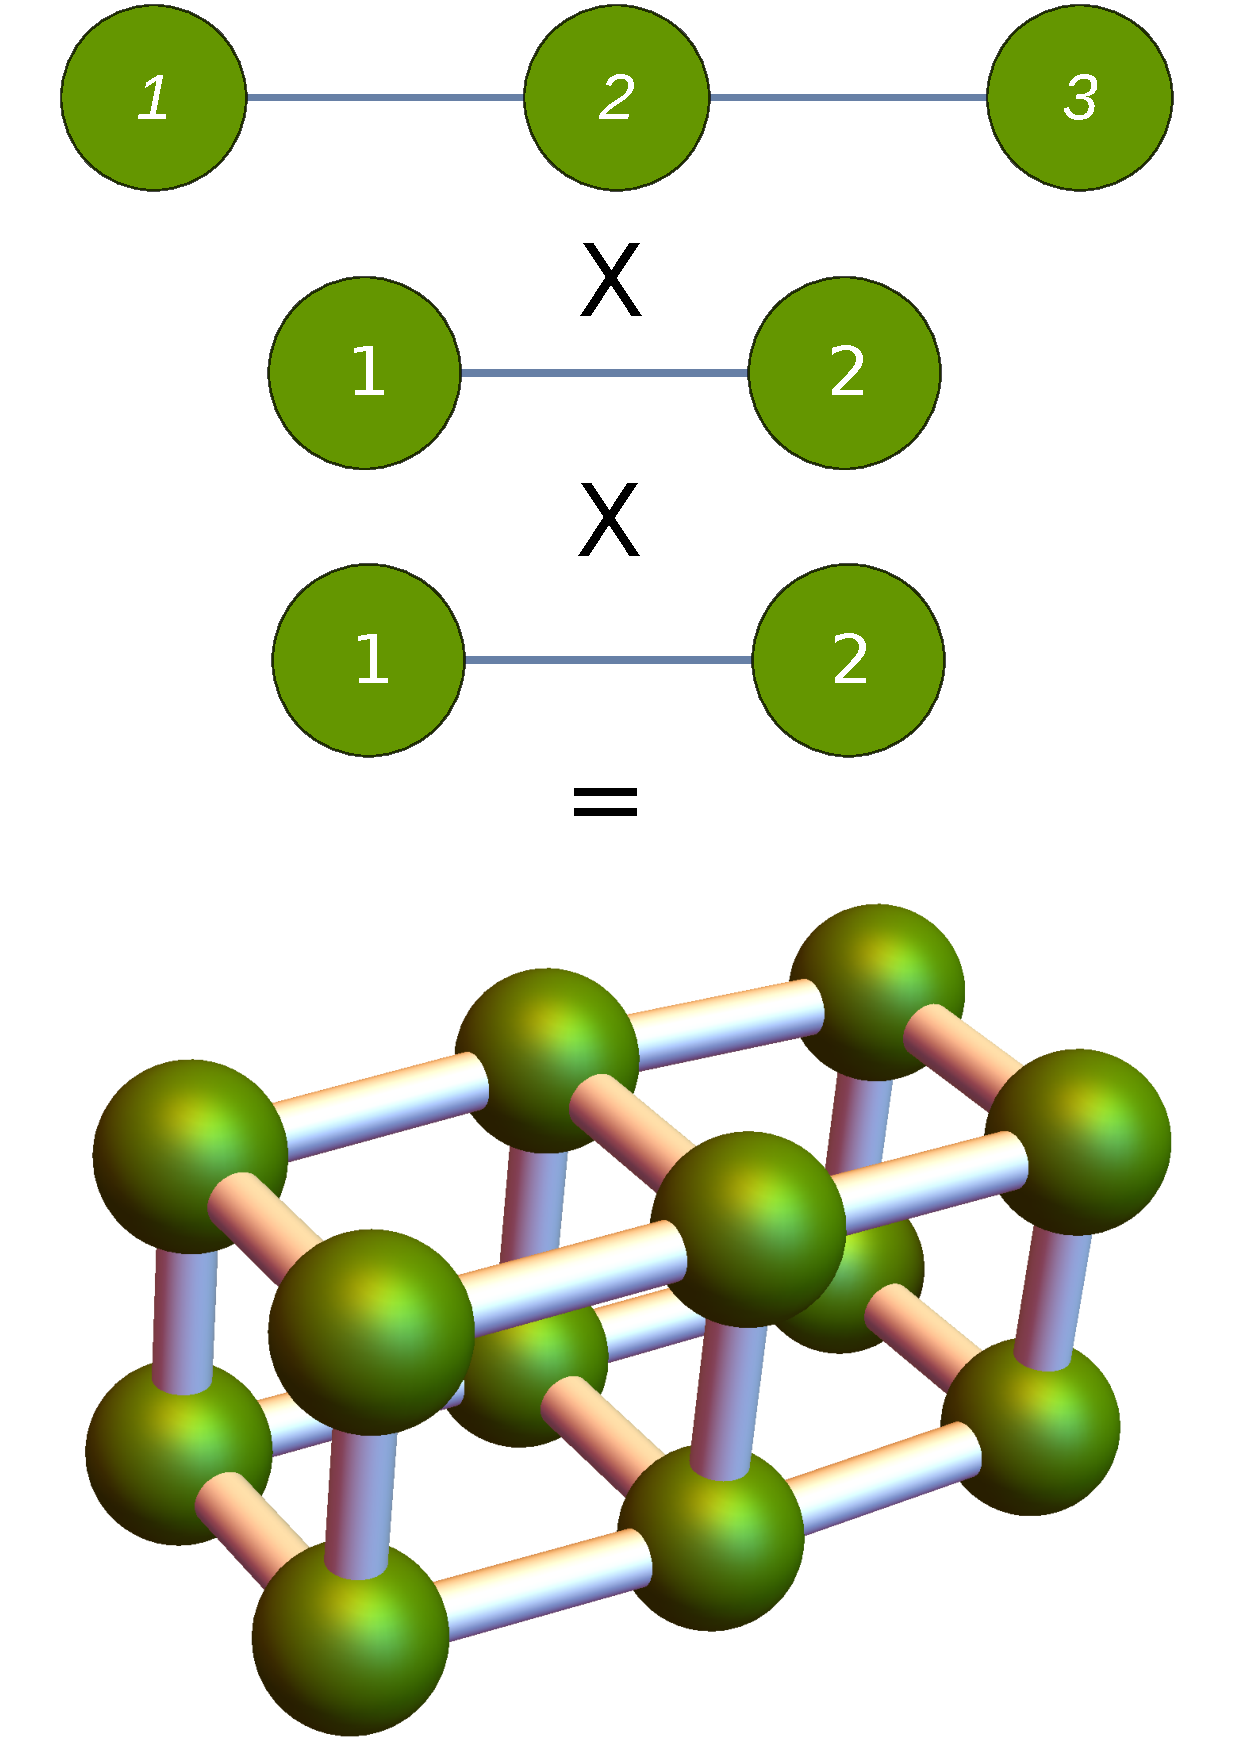
\includegraphics[trim=0mm 0 0 0mm, width=1.0\textwidth]{Images/graphprod_chain3_chain2_square} \\
		\end{column}
		\begin{column}{0.33\textwidth}
			\centering
   			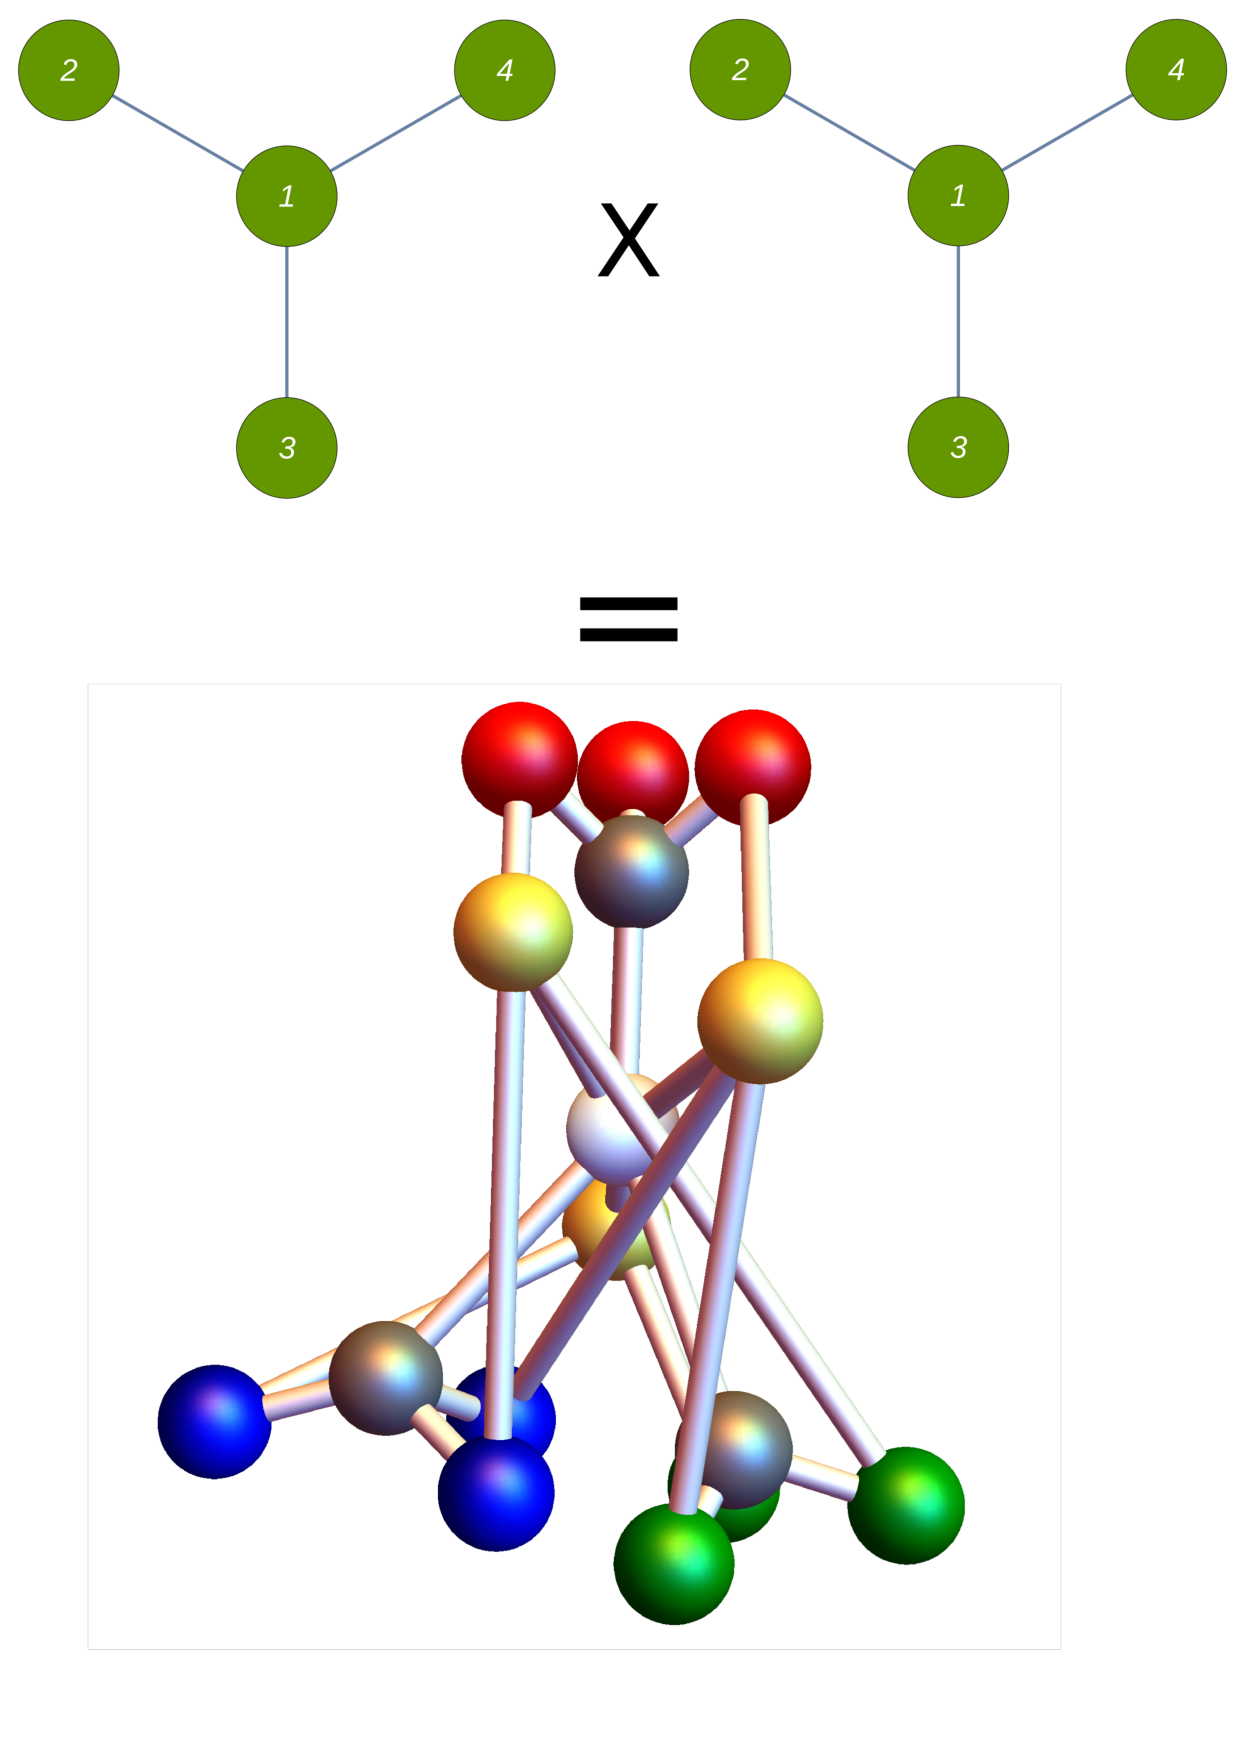
\includegraphics[trim=0mm 0 0 0mm, width=1.0\textwidth]{Images/graphprod_switch_square.pdf} 
		\end{column}
	\end{columns}
\end{frame}}	
	
\begin{center}
	\includeslide{complexity}
\end{center}

\noindent text



\section{Perfect State Transfer}

\subsection{PST}

\mode<presentation>{\begin{frame}{Perfect State Transfer}\label{pst}
	\centering\vspace*{0.4cm}
	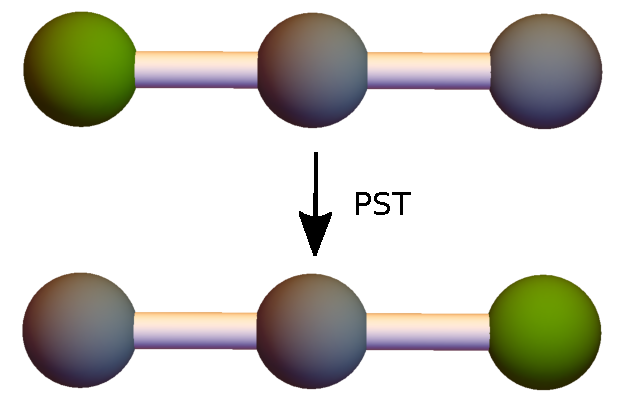
\includegraphics[trim=-5mm 0 0 0mm, width=0.45\textwidth]{Images/chain3-pst-marked-start-and-end}
	\vspace*{-0.4cm}
	\begin{exampleblock}{}
	\setlength\abovedisplayskip{-8pt}
	\begin{center}
		\[ \left|f^N_{r,s}(t)\right| = \left|\bra{r}\text{e}^{-\text{i}H t}\ket{s}\right| \mbeq 1 \]
	\end{center}
	\end{exampleblock}\vspace*{-0.4cm}
	\begin{exampleblock}{}
	\setlength\abovedisplayskip{-8pt}
	\begin{center}
		$ f^{\left|V_{G\times H}\right|}_{(r,r'),(s,s')}(t) = f^{\left|V_G\right|}_{r,s}(t)\cdot f^{\left|V_H\right|}_{r',s'}(t) $
	\end{center}
	\end{exampleblock}
\end{frame}}

\begin{center}
	\includeslide{qubits}
\end{center}

\noindent text

\mode<presentation>{\begin{frame}{Binary Numbers}\label{bns}
	\centering\vspace*{0.3cm}
	\begin{itemize}
		\item Prepare qubit $2$ as $\ket{\psi} = \alpha\ket{0} + \beta\ket{1}$
		\item Register is $\ket{\Psi} = \alpha\ket{0000} + \beta\ket{0100}$
		\item States as vectors:
			\[ \ket{0100} = 
				\begin{pmatrix}
					0 \\
					1 \\
					0 \\
					0 
				\end{pmatrix} \quad \text{etc.} \]
	\end{itemize}
	\begin{exampleblock}{}
	\setlength\abovedisplayskip{-8pt}
	\begin{center}
		\[ \text{PST} \rightarrow \text{e}^{-\text{i}H \tau} = P_\pi \]
	\end{center}
	\end{exampleblock}
\end{frame}}

\begin{center}
	\includeslide{PST}
\end{center}

\noindent text


\subsection{Detecting PST}
\mode<presentation>{\begin{frame}[t]{Detecting PST}\label{detectingpst}
	\begin{exampleblock}{}
	\setlength\abovedisplayskip{-8pt}
	\begin{center}
		\[ P_\pi^T P_\pi = 1 \rightarrow \text{e}^{-\text{i}H 2\tau} \mbeq 1 \]
	\end{center}
	\end{exampleblock}
	\vspace*{0.7cm}
	Generalized:
	\begin{columns}[T]
		\begin{column}{0.5\textwidth}
			\centering
			\[ \text{e}^{-\text{i}H 2\tau} =
			\begin{pmatrix}
				\text{e}^{\text{i}\phi} & 0 & 0 & 0 \\
				0 & \text{e}^{\text{i}\phi} & 0 & 0 \\
				0 & 0 & a & b \\
				0 & 0 & c & d 
			\end{pmatrix} \] 
		\end{column}
		\begin{column}{0.5\textwidth}
			\centering
   			\[ P_\pi =
			\begin{pmatrix}
				0 & \text{e}^{\text{i}\theta} & 0 & 0 \\
				\text{e}^{\text{i}\theta} & 0 & 0 & 0 \\
				0 & 0 & \hat{a} & \hat{b} \\
				0 & 0 & \hat{c} & \hat{d} 
			\end{pmatrix} \]
		\end{column}
	\end{columns}
\end{frame}}


\section{Spin Networks}

\subsection{Spin Chains}

\mode<presentation>{\begin{frame}[t]{Spin Chains}\label{spinchains}
	\begin{columns}[T]
		\begin{column}{0.5\textwidth}
			\centering\vspace*{0.2cm}
			
\includegraphics[trim=-5mm 0 0 0mm, width=0.8\textwidth]{Images/chain2-graph}\vspace*{0.4cm} \\
			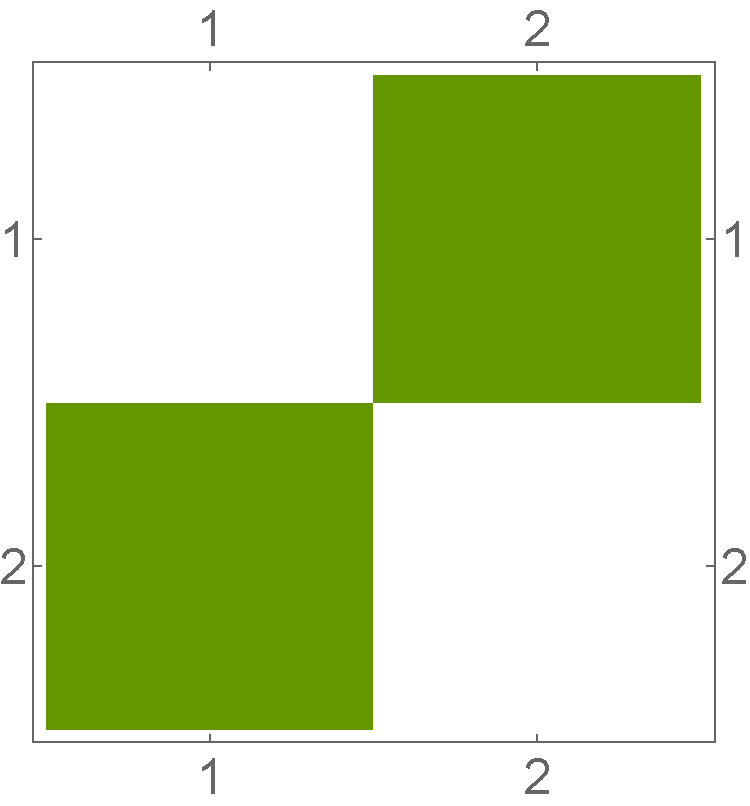
\includegraphics[trim=-5mm 0 0 0mm, width=0.8\textwidth]{Images/chain2_pqst} \\
			$\tau_{c2} = \frac{\pi}{2}$
		\end{column}
		\begin{column}{0.5\textwidth}
			\centering\vspace*{0.2cm}
   			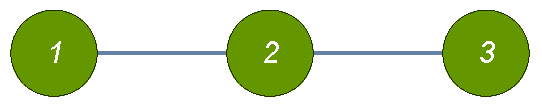
\includegraphics[trim=-5mm 0 0 0mm, width=1.0\textwidth]{Images/chain3-graph}\vspace*{0.55cm} \\
   			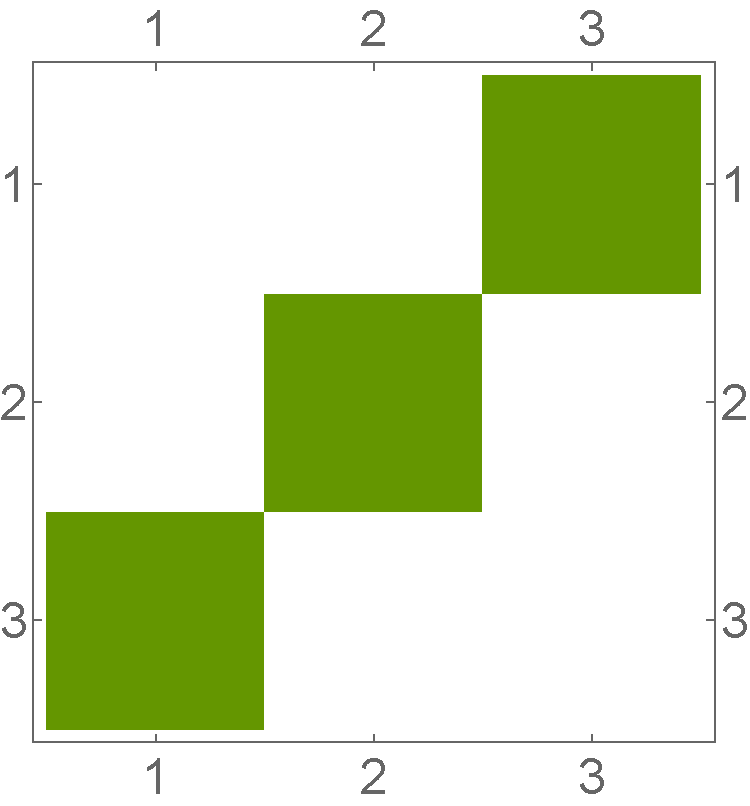
\includegraphics[trim=-5mm 0 0 0mm, width=0.8\textwidth]{Images/chain3_pqst} \\
   			$\tau_{c3} = \frac{\pi}{\sqrt{2}}$
		\end{column}
	\end{columns}\vspace*{0.3cm}
	\footnotesize\textcolor{tugreen}{$\blacktriangleright$}\,\,\cite{Christandl2004}\normalsize
\end{frame}}

\begin{center}
	\includeslide{qregister}
\end{center}

\noindent text


\mode<presentation>{\begin{frame}[t]{Spin Hypercubes}\label{spinhypercubes}
	\begin{columns}[T]
		\begin{column}{0.5\textwidth}
			\centering\vspace*{0.2cm}
			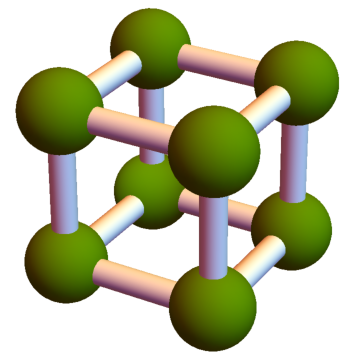
\includegraphics[trim=-5mm 0 0 0mm, width=0.4\textwidth]{Images/chain2-cube} \\
			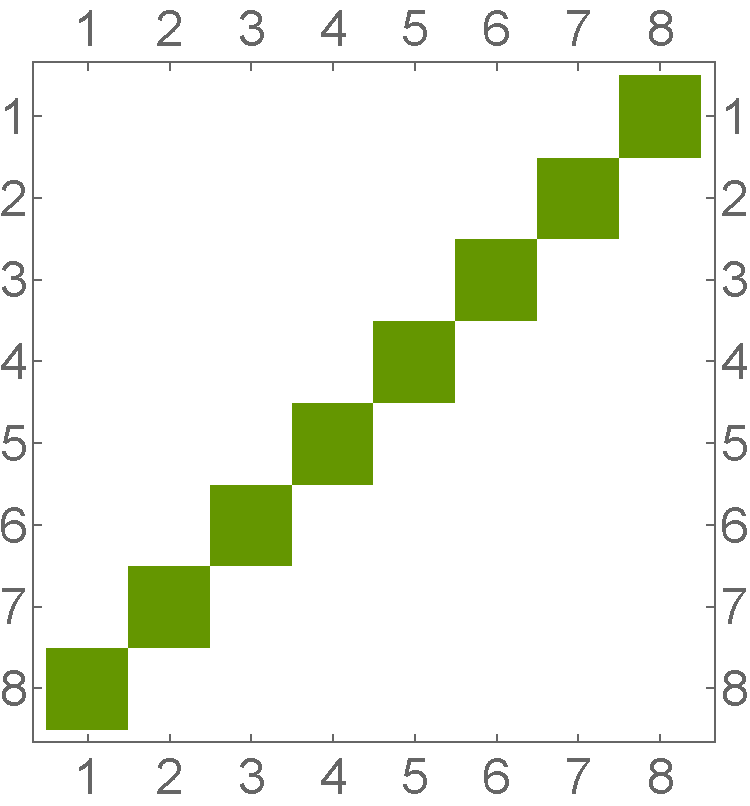
\includegraphics[trim=-5mm 0 0 0mm, width=0.8\textwidth]{Images/chain2-cube-permutation} \\
			$\tau_{c2} = \frac{\pi}{2}$
		\end{column}
		\begin{column}{0.5\textwidth}
			\centering\vspace*{0.2cm}
   			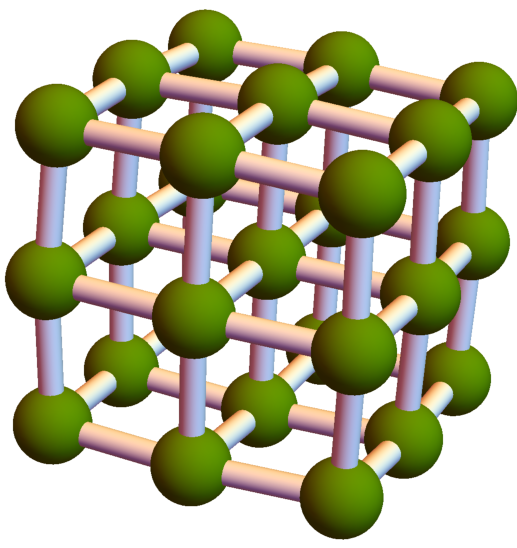
\includegraphics[trim=-5mm 0 0 0mm, width=0.35\textwidth]{Images/chain3-cube} \\
   			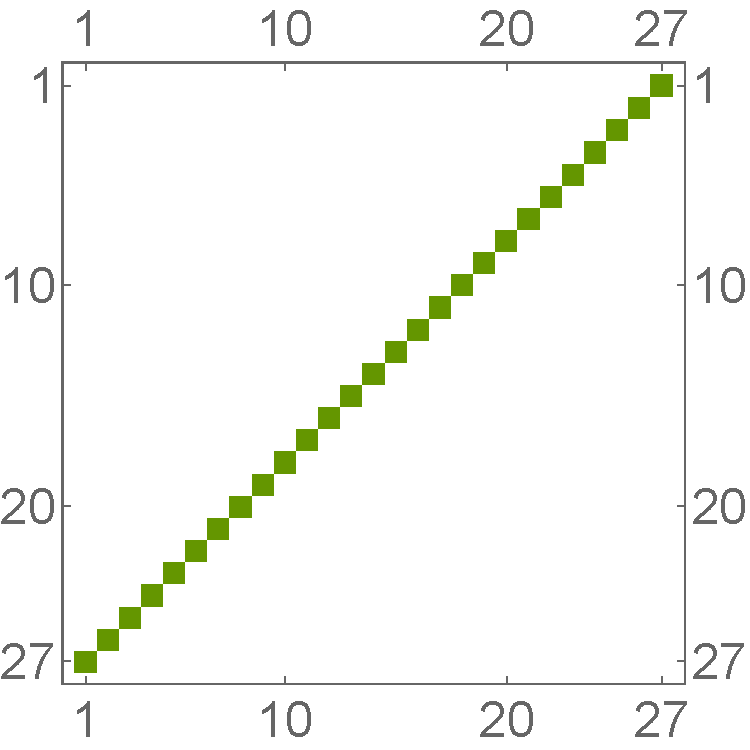
\includegraphics[trim=-5mm 0 0 0mm, width=0.9\textwidth]{Images/chain3-cube-permutation} \\
   			$\tau_{c3} = \frac{\pi}{\sqrt{2}}$
		\end{column}
	\end{columns}\vspace*{0.3cm}
	\footnotesize\textcolor{tugreen}{$\blacktriangleright$}\,\,\cite{Christandl2004}\normalsize
\end{frame}}

\begin{center}
	\includeslide{qregister}
\end{center}

\noindent text


\subsection{Quantum Routing}

\mode<presentation>{\begin{frame}[t]{Quantum Routing}\label{quantumrouting}
	\begin{exampleblock}{}
	\setlength\abovedisplayskip{-8pt}
	\begin{center}
		\[ H = \frac{1}{2}J\sum_{i=2}^{N}\left[\sigma_1^x\sigma_i^x + \sigma_1^y\sigma_i^y\right] + \sum_{i=1}^{N}h_i\sigma_i^z \]
	\end{center}
	\end{exampleblock}
	\begin{columns}[T]
		\begin{column}{0.5\textwidth}
		\begin{center}
			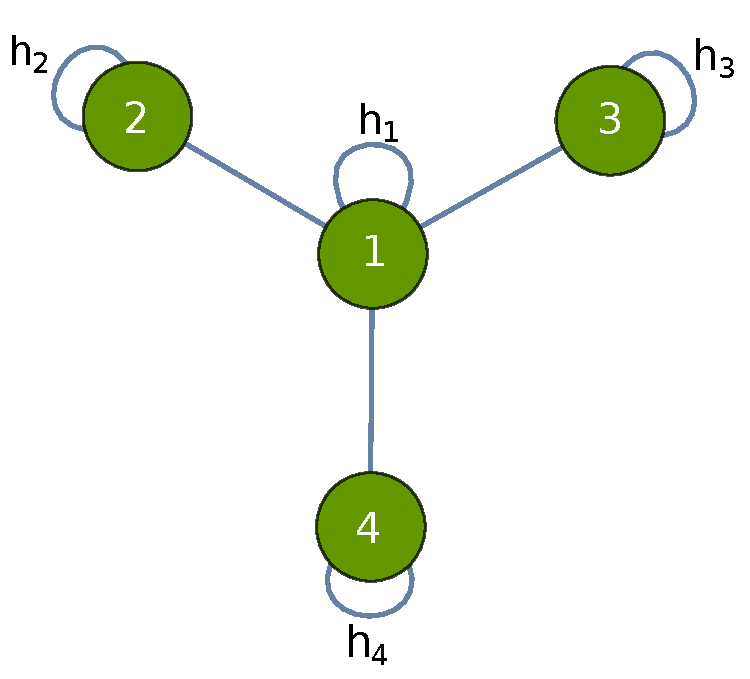
\includegraphics[trim=0mm 0 0 20mm, width=0.85\textwidth]{Images/switch_selfloops}
		\end{center}
		\end{column}
		\begin{column}{0.5\textwidth}
		\begin{center}
			\vspace*{0.5cm}
			\begin{itemize}
				\item Local potentials $h_i$
				\item Field at each node
				\item Apply global offset field
				\item More arms are possible
			\end{itemize}
		\end{center}
		\end{column}
	\end{columns}
	\vspace*{0.2cm}
	\footnotesize\textcolor{tugreen}{$\blacktriangleright$}\,\,\cite{Yung2011}\normalsize
\end{frame}}

\begin{center}
	\includeslide{quantum parallel}
\end{center}

\noindent text


\mode<presentation>{\begin{frame}{Spin Switch}\label{switch}
	\vspace*{0.5cm}
	\centering
	\begin{center}
		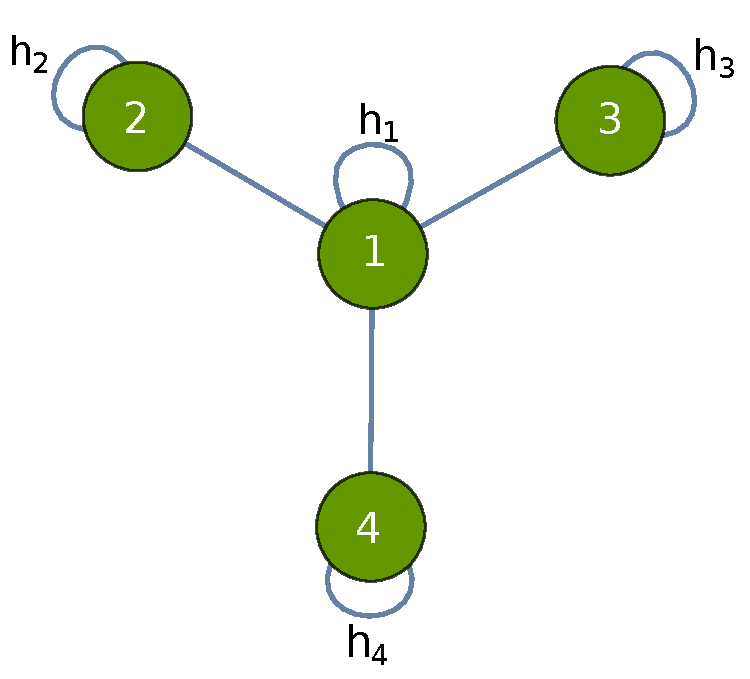
\includegraphics[trim=0mm 0 0 10mm, width=0.35\textwidth]{Images/switch_selfloops}
	\end{center}\vspace*{-0.75cm}
	\begin{columns}[T]
		\begin{column}{0.5\textwidth}
		\begin{center}
			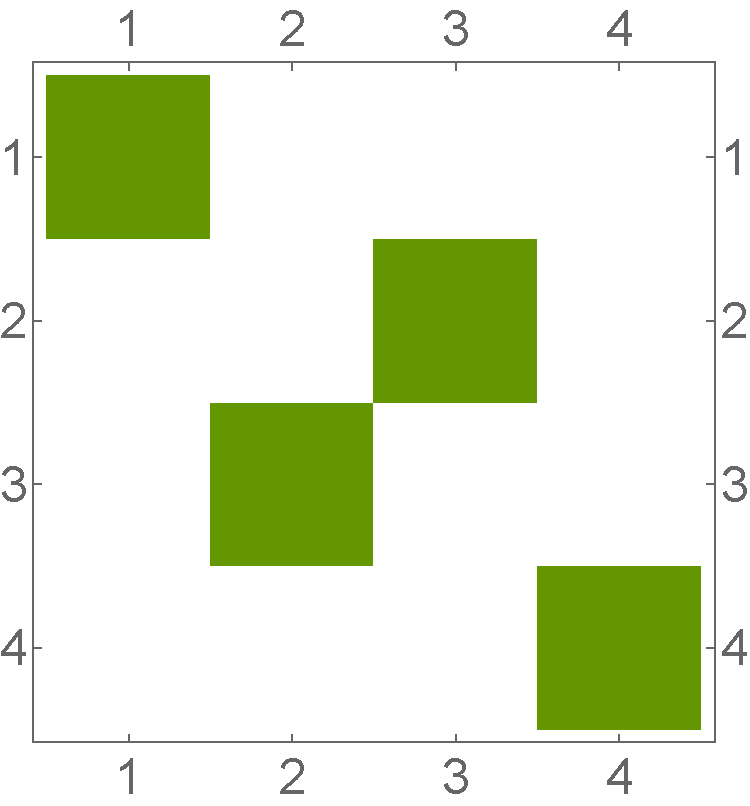
\includegraphics[trim=0mm 0 0 10mm, width=0.65\textwidth]{Images/switch-permutation}
		\end{center}
		\end{column}
		\begin{column}{0.5\textwidth}
		\begin{center}
			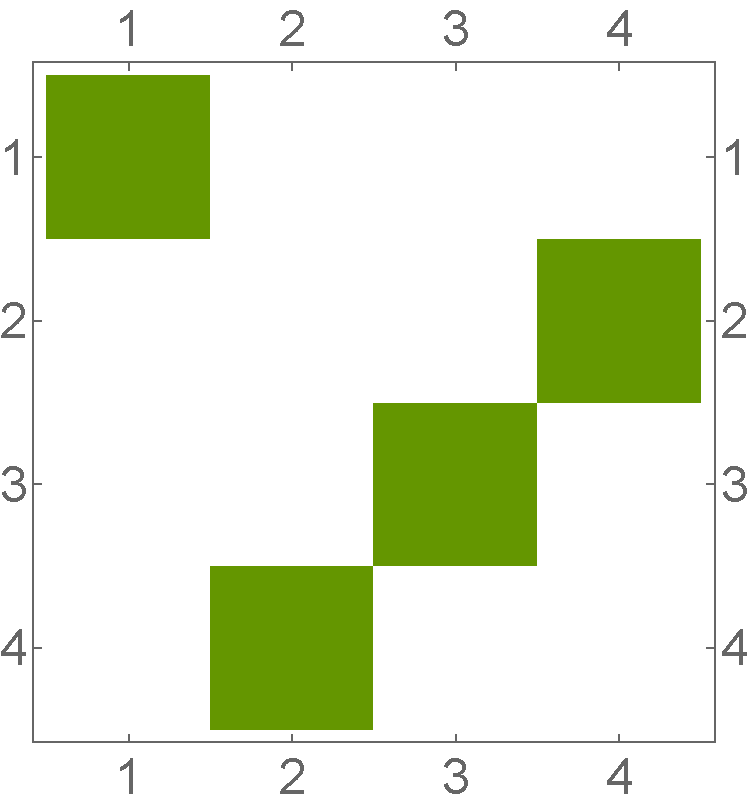
\includegraphics[trim=0mm 0 0 10mm, width=0.65\textwidth]{Images/switch2-permutation}
		\end{center}
		\end{column}
	\end{columns}
	$\tau_{s3} = \frac{\pi}{0.766}$
\end{frame}}

\begin{center}
	\includeslide{qft}
\end{center}

\noindent text


\mode<presentation>{\begin{frame}{Spin Switch}\label{switchsquare}
	\vspace*{0.5cm}
	\centering
	\begin{center}
		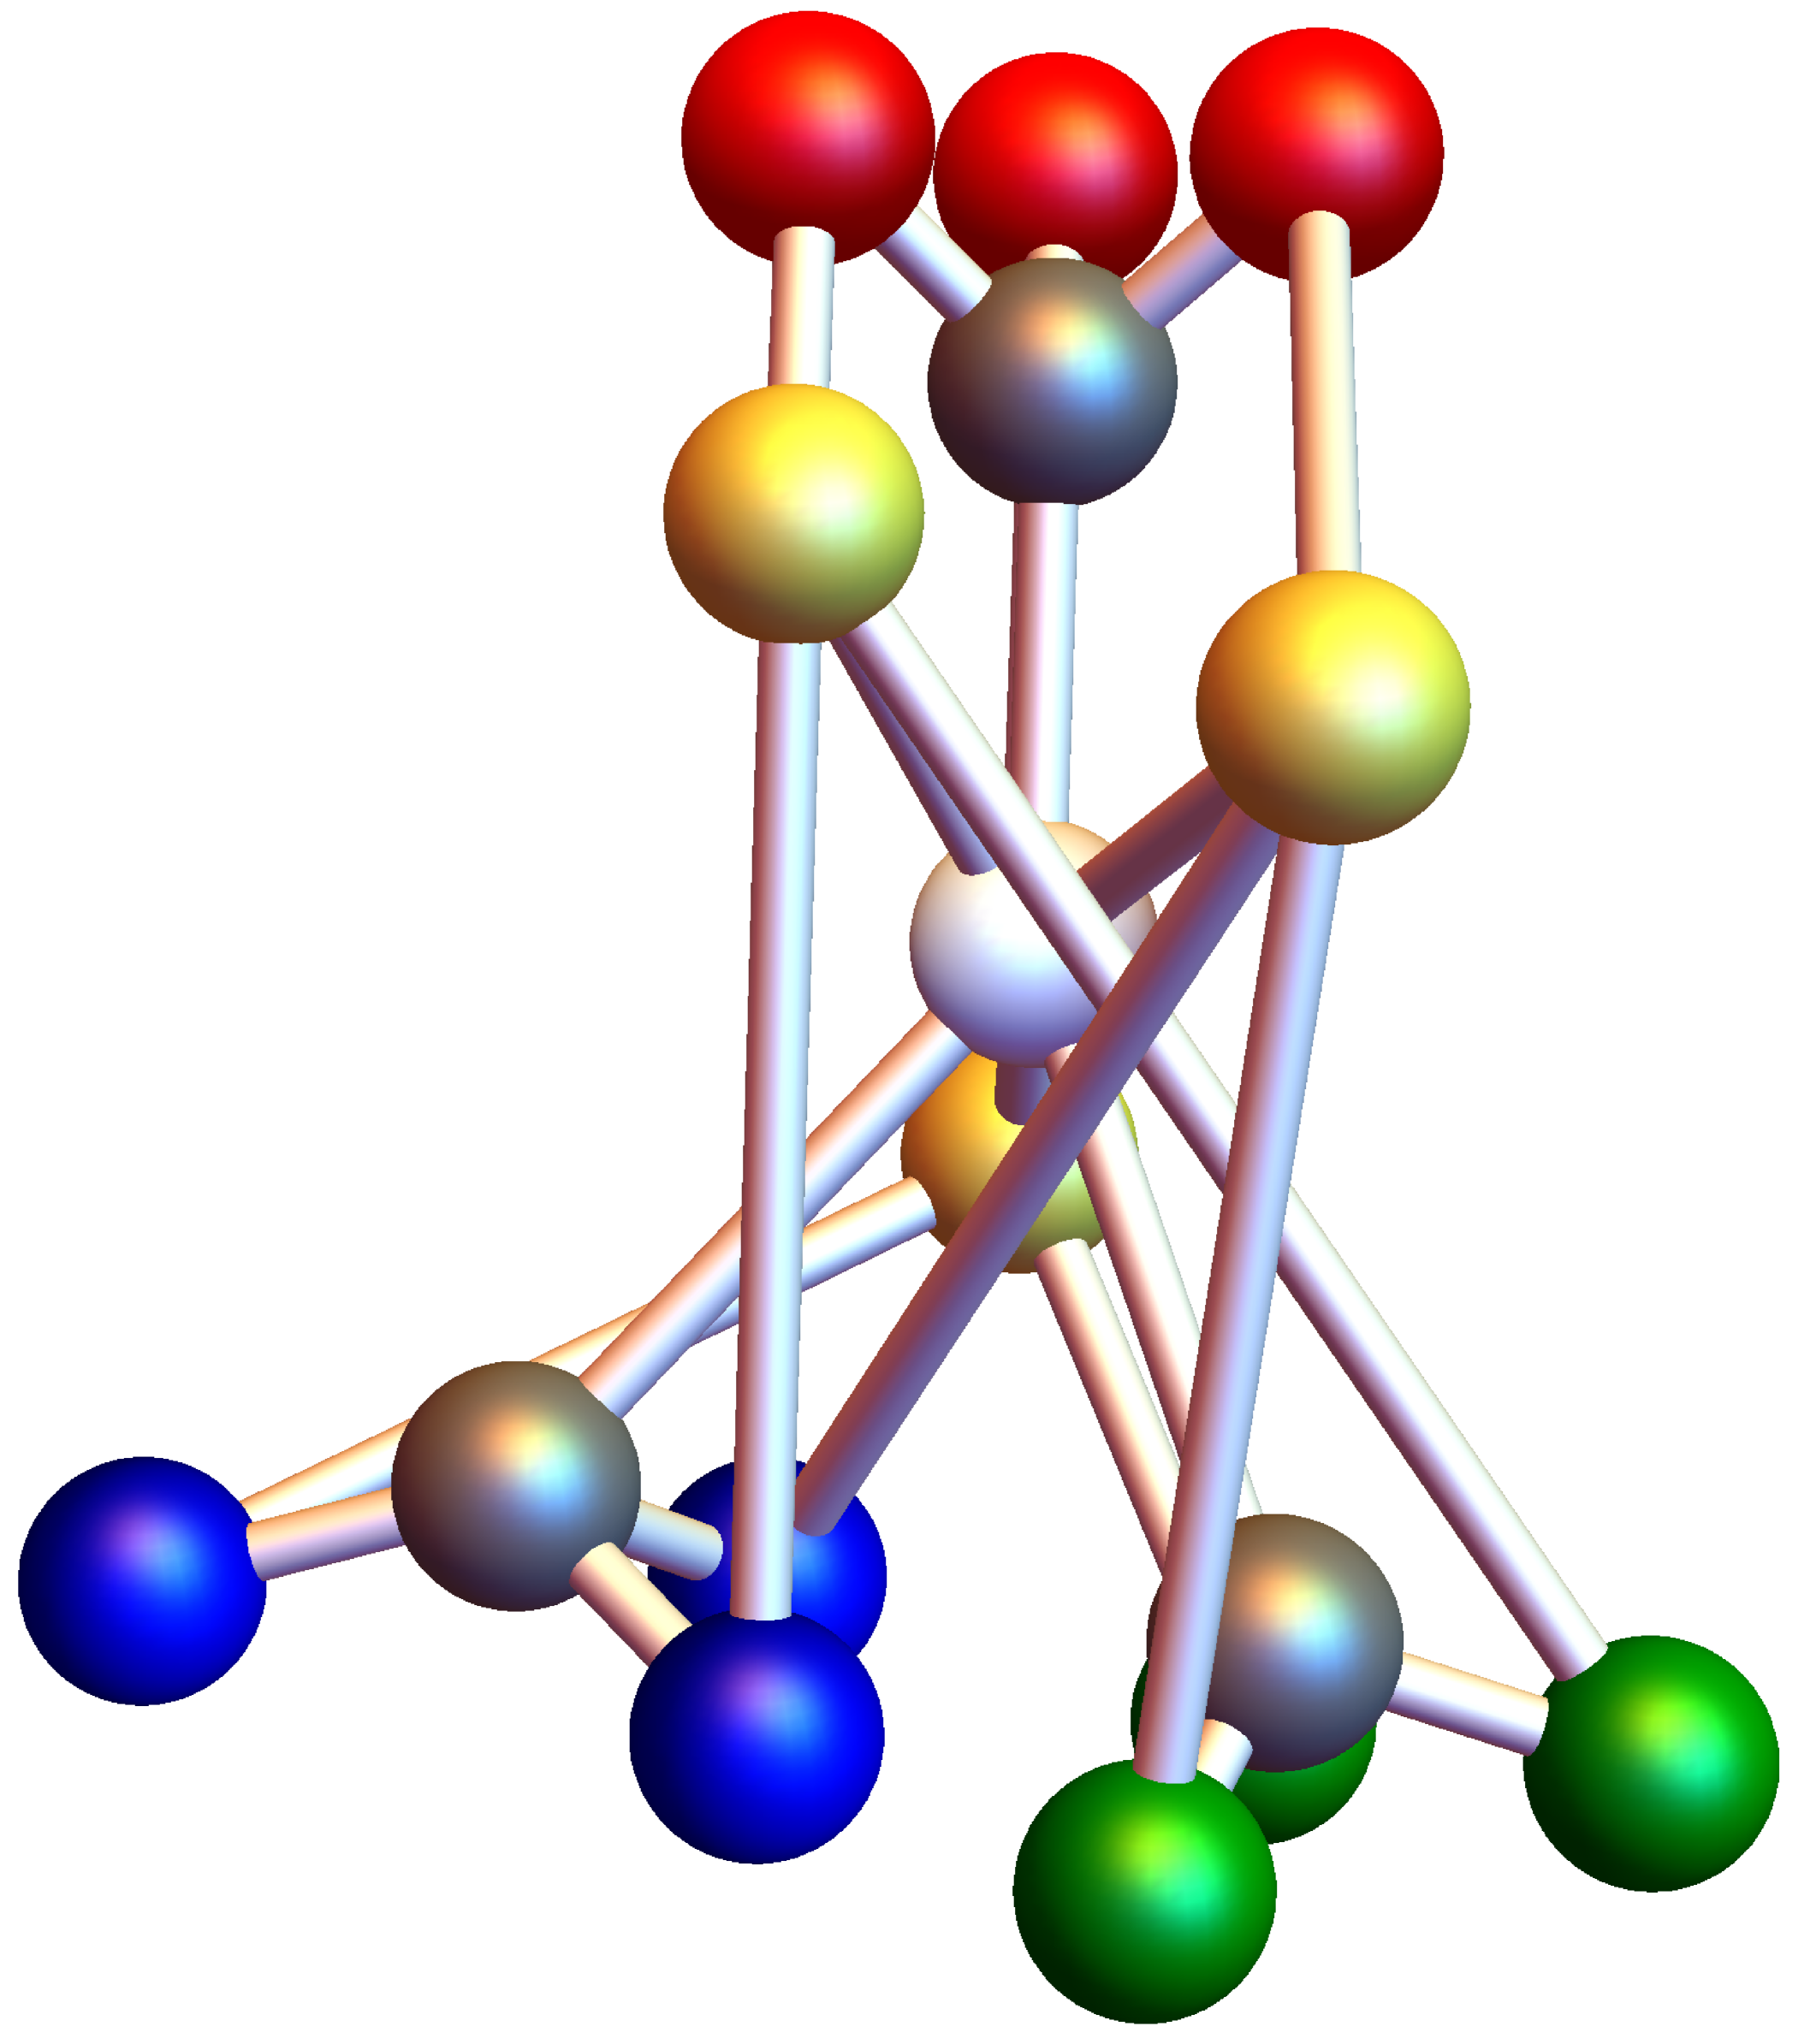
\includegraphics[trim=0mm 0 0 10mm, width=0.29\textwidth]{Images/switch_square.png}
	\end{center}\vspace*{-0.75cm}
	\begin{columns}[T]
		\begin{column}{0.5\textwidth}
		\begin{center}
			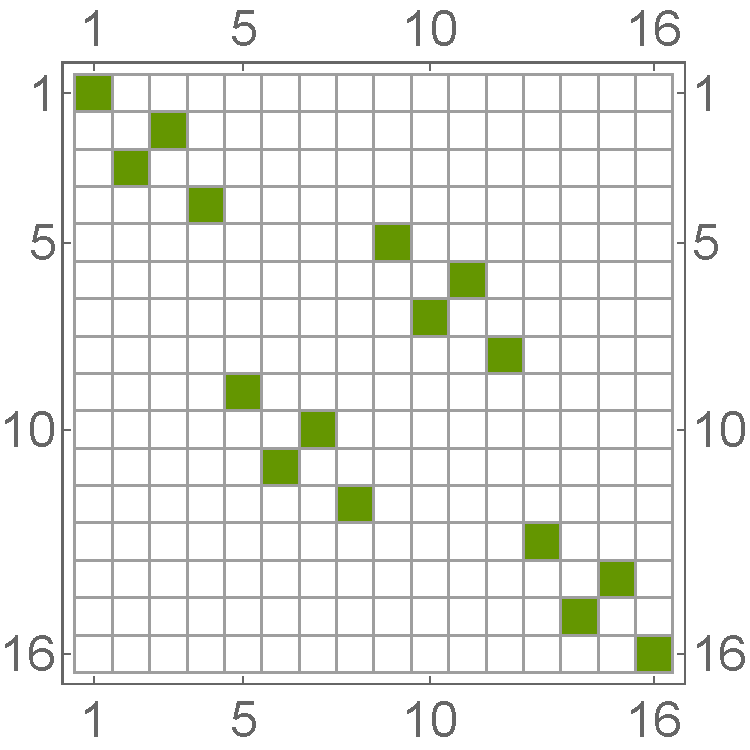
\includegraphics[trim=0mm 0 0 10mm, width=0.65\textwidth]{Images/switchsquare-permutation}
		\end{center}
		\end{column}
		\begin{column}{0.5\textwidth}
		\begin{center}
			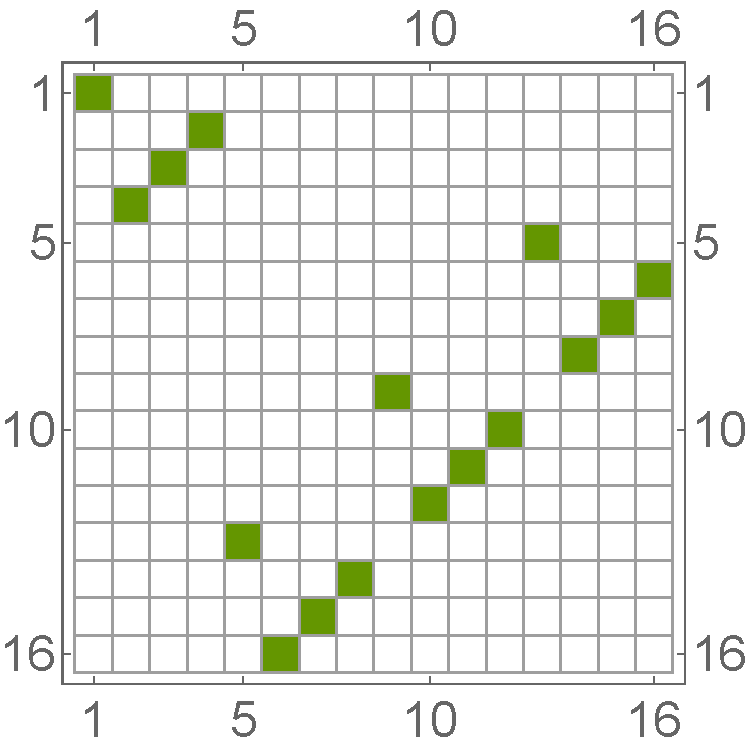
\includegraphics[trim=0mm 0 0 10mm, width=0.65\textwidth]{Images/switchsquare2-permutation}
		\end{center}
		\end{column}
	\end{columns}
	$\tau_{s3} = \frac{\pi}{0.766}$
\end{frame}}

\begin{center}
	\includeslide{qft}
\end{center}

\noindent text


\section{Designing Spin Networks}

\subsection{Renormalization}

\mode<presentation>{\begin{frame}[t]{Renormalization}\label{renormalization}
	\begin{columns}[T]
		\begin{column}{0.5\textwidth}
		\begin{center}
			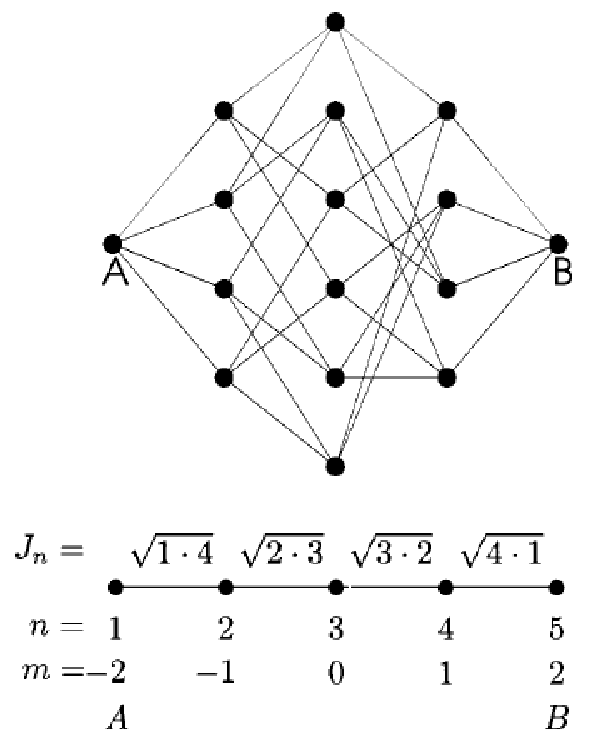
\includegraphics[trim=0mm 0 0 10mm, width=0.9\textwidth]{Images/hypercube-to-perfect-couplings} \\
			$\tau_{c5p} = \frac{\pi}{2}$
		\end{center}
		\end{column}
		\begin{column}{0.5\textwidth}
		\begin{center}
			\uncover<2->{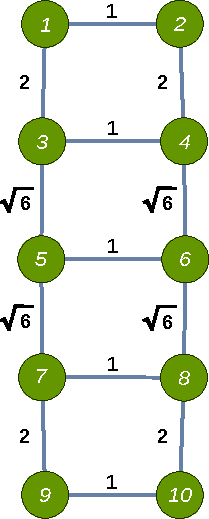
\includegraphics[trim=0mm 0 0 10mm, width=0.5\textwidth]{Images/pc-spin-ladder-graph}}
		\end{center}
		\end{column}
	\end{columns}	
	\vspace*{0.45cm}
	\footnotesize\textcolor{tugreen}{$\blacktriangleright$}\,\,\cite{Christandl2004}\normalsize
\end{frame}}

\begin{center}
	\includeslide{amplification}
\end{center}

\noindent text



\mode<presentation>{\begin{frame}{Reverse Renormalization}\label{reverserenormalization}
	\begin{columns}[T]
		\begin{column}{0.5\textwidth}
			\centering\vspace*{1cm}
			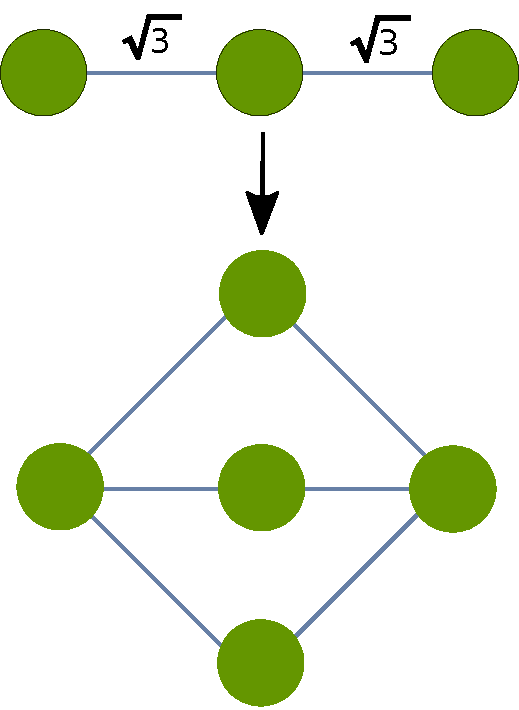
\includegraphics[trim=0mm 0 0 10mm, width=0.85\textwidth]{Images/eg-renorm-3}
		\end{column}		
		\begin{column}{0.5\textwidth}
			\centering
			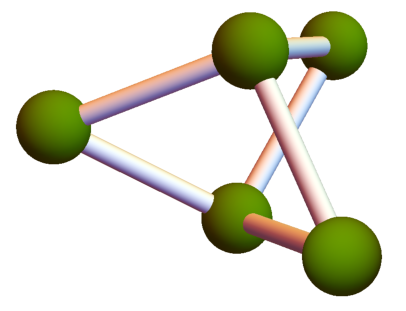
\includegraphics[trim=0 0 0 0mm, width=0.4\textwidth]{Images/eg-triplearmstar-uniform} \\
			$\tau_{s3} = \frac{\pi}{\sqrt{6}}$ \\
			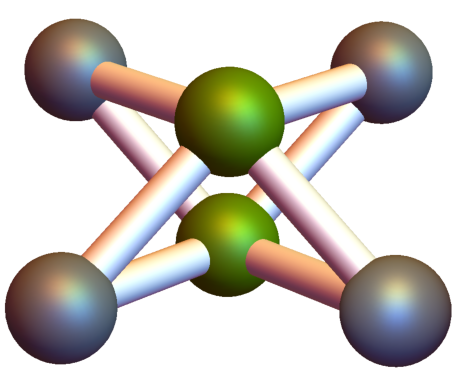
\includegraphics[trim=0 0 0 0mm, width=0.4\textwidth]{Images/chain2square-hes2-pst-marked} \\
			$\tau_{s4} = \frac{\pi}{\sqrt{8}}$ \\
			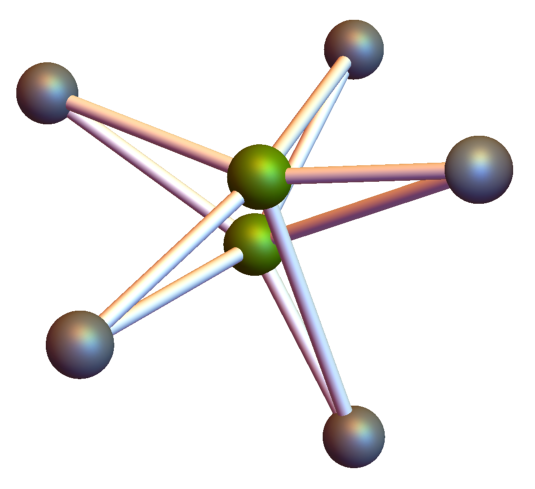
\includegraphics[trim=0 0 0 0mm, width=0.4\textwidth]{Images/eg-pentaarmstar-uniform} \\
			$\tau_{s5} = \frac{\pi}{\sqrt{10}}$
		\end{column}
	\end{columns}
\end{frame}}

\begin{center}
	\includeslide{qrw}
\end{center}

\noindent text



\subsection{Higher Excitation Spaces}

\mode<presentation>{\begin{frame}[t]{Higher Excitation Spaces}\label{hes}
	\centering
	\begin{columns}[T]
		\begin{column}{0.5\textwidth}
			\centering
			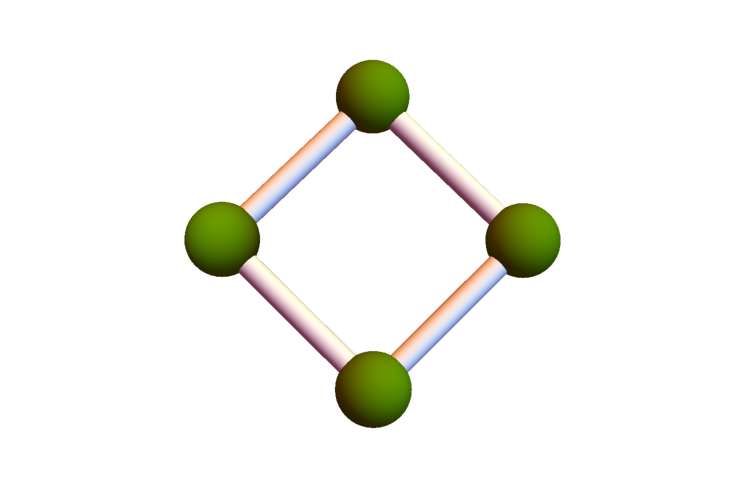
\includegraphics[trim=0 0 0 0mm, width=0.9\textwidth]{Images/method4-solution-chain2square} \\
			\vspace*{0.3cm}
			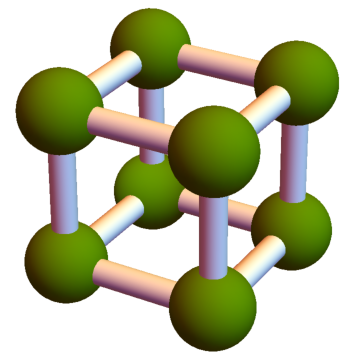
\includegraphics[trim=0 0 0 0mm, width=0.7\textwidth]{Images/chain2-cube}
		\end{column}		
		\begin{column}{0.5\textwidth}
			\centering
			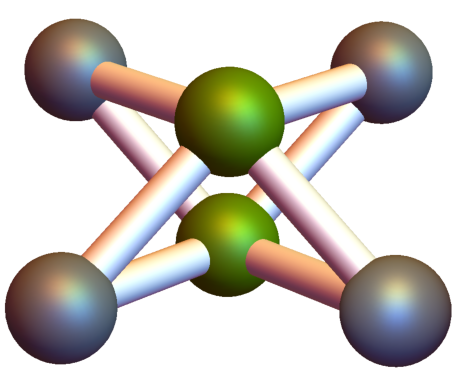
\includegraphics[trim=0 0 0 0mm, width=0.7\textwidth]{Images/chain2square-hes2-pst-marked} \\
			\vspace*{0.5cm}
			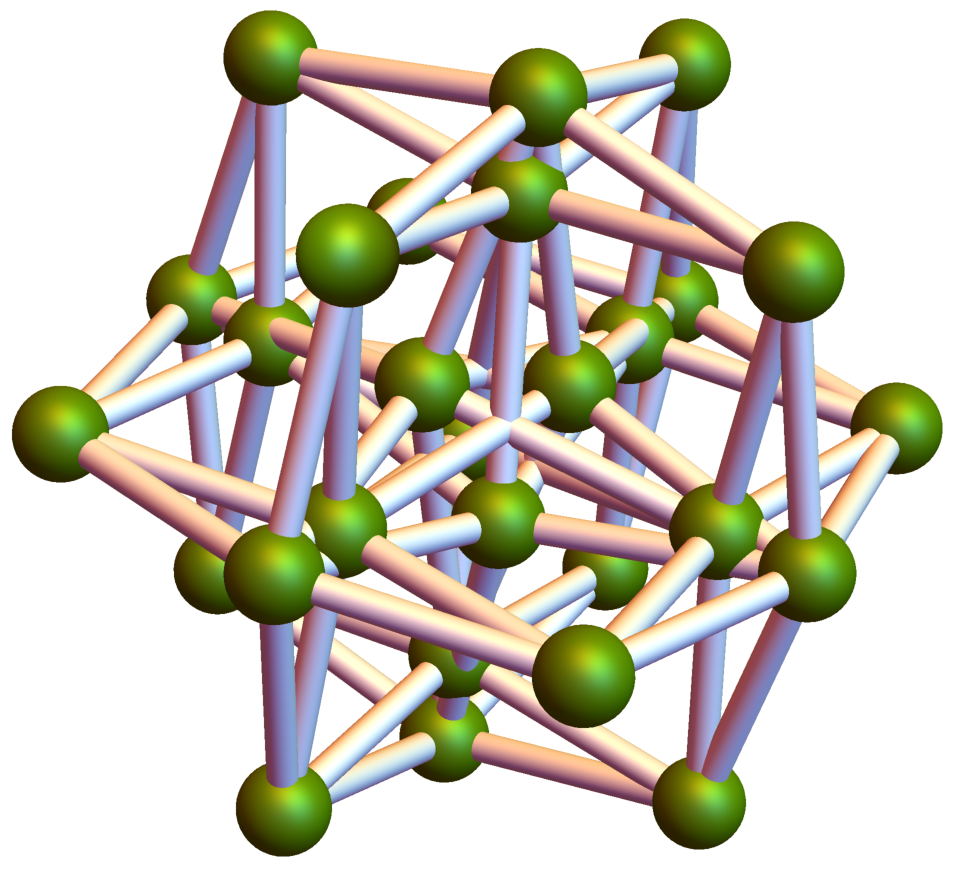
\includegraphics[trim=0 0 0 0mm, width=0.7\textwidth]{Images/chain2cube-hes2}
		\end{column}
	\end{columns}
\end{frame}}


\begin{center}
	\includeslide{strengths}
\end{center}

\noindent text


\mode<presentation>{\begin{frame}[t]{Higher Excitation Spaces}\label{hes}
	\centering
	\Large
	\begin{table}
		\begin{tabular}{l | c }
			Task & Complexity \\
			\hline \hline
			Discrete log & $\mathcal{O}(n^3)$ \\
			Verify MatMult & $\mathcal{O}(n^\frac{5}{3})$ \\
			$k$ Fake Coins & $\mathcal{O}(k^\frac{1}{4})$ \\
			Factorization & $\mathcal{O}(n^3)$ \\
			List search & $\mathcal{O}(\sqrt{n})$ 
		\end{tabular}
	%\caption{Complexity}
	\end{table}
	\normalsize
	\begin{itemize}
		\item Optimization
		\item Big Data
		\item Artificial Intelligence
	\end{itemize}
	\vspace*{0.5cm}
	See \textsc{NIST} Quantum Algorithm Zoo for more
\end{frame}}


\begin{center}
	\includeslide{strengths}
\end{center}

\noindent text



\subsection{Realization}

\mode<presentation>{\begin{frame}[t]{D-Wave 2000Q}\label{dwave}
	\begin{columns}[T]
		\begin{column}{0.5\textwidth}
			\centering
			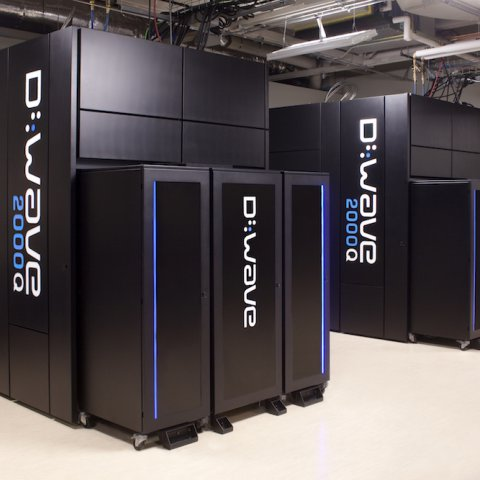
\includegraphics[trim=0 0 0 0mm, width=0.75\textwidth]{Images/d-wave2000q.jpg} \\
			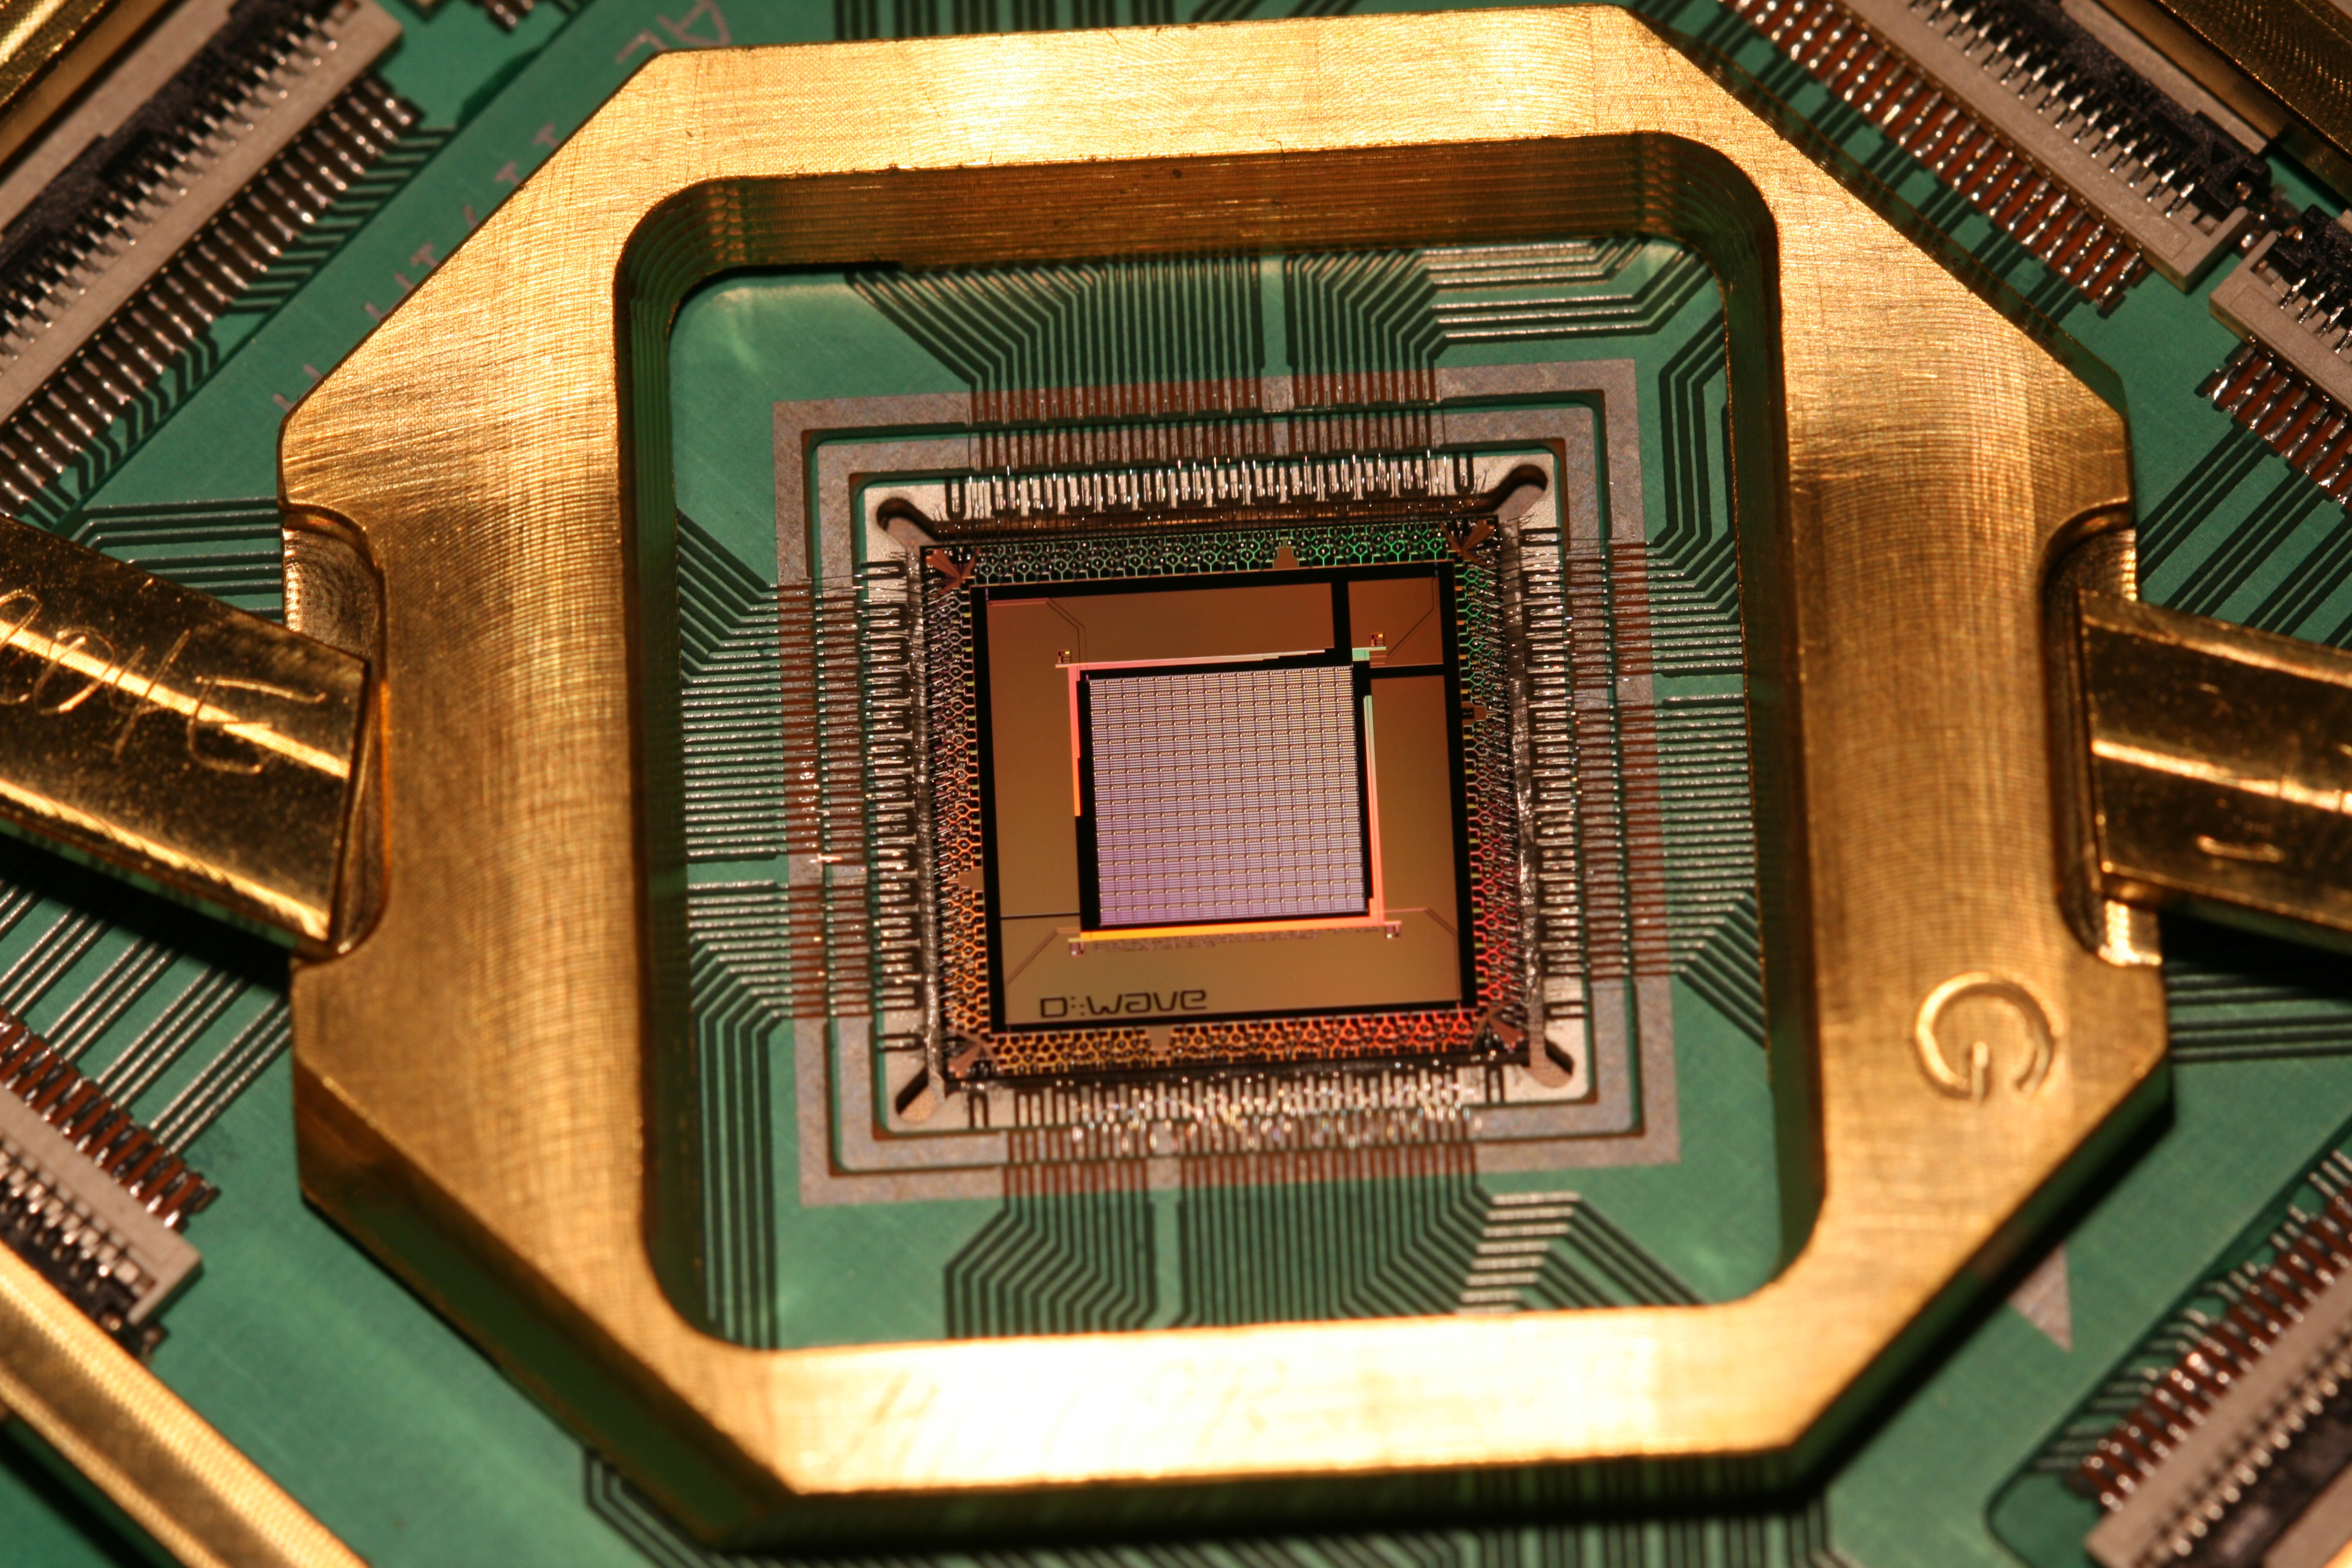
\includegraphics[trim=0 0 0 0mm, width=0.75\textwidth]{Images/d-wave-processor.jpg}
		\end{column}
		\begin{column}{0.5\textwidth}
			\centering
			\begin{itemize}
				\item Quantum Annealer
				\item $2000$ squids 
				\item $25$\,kW vs. $\mathcal{O}(1000)$\,kW
				\item Temperature $0.015$\,K
			\end{itemize}
			\vspace*{0.5cm}
    		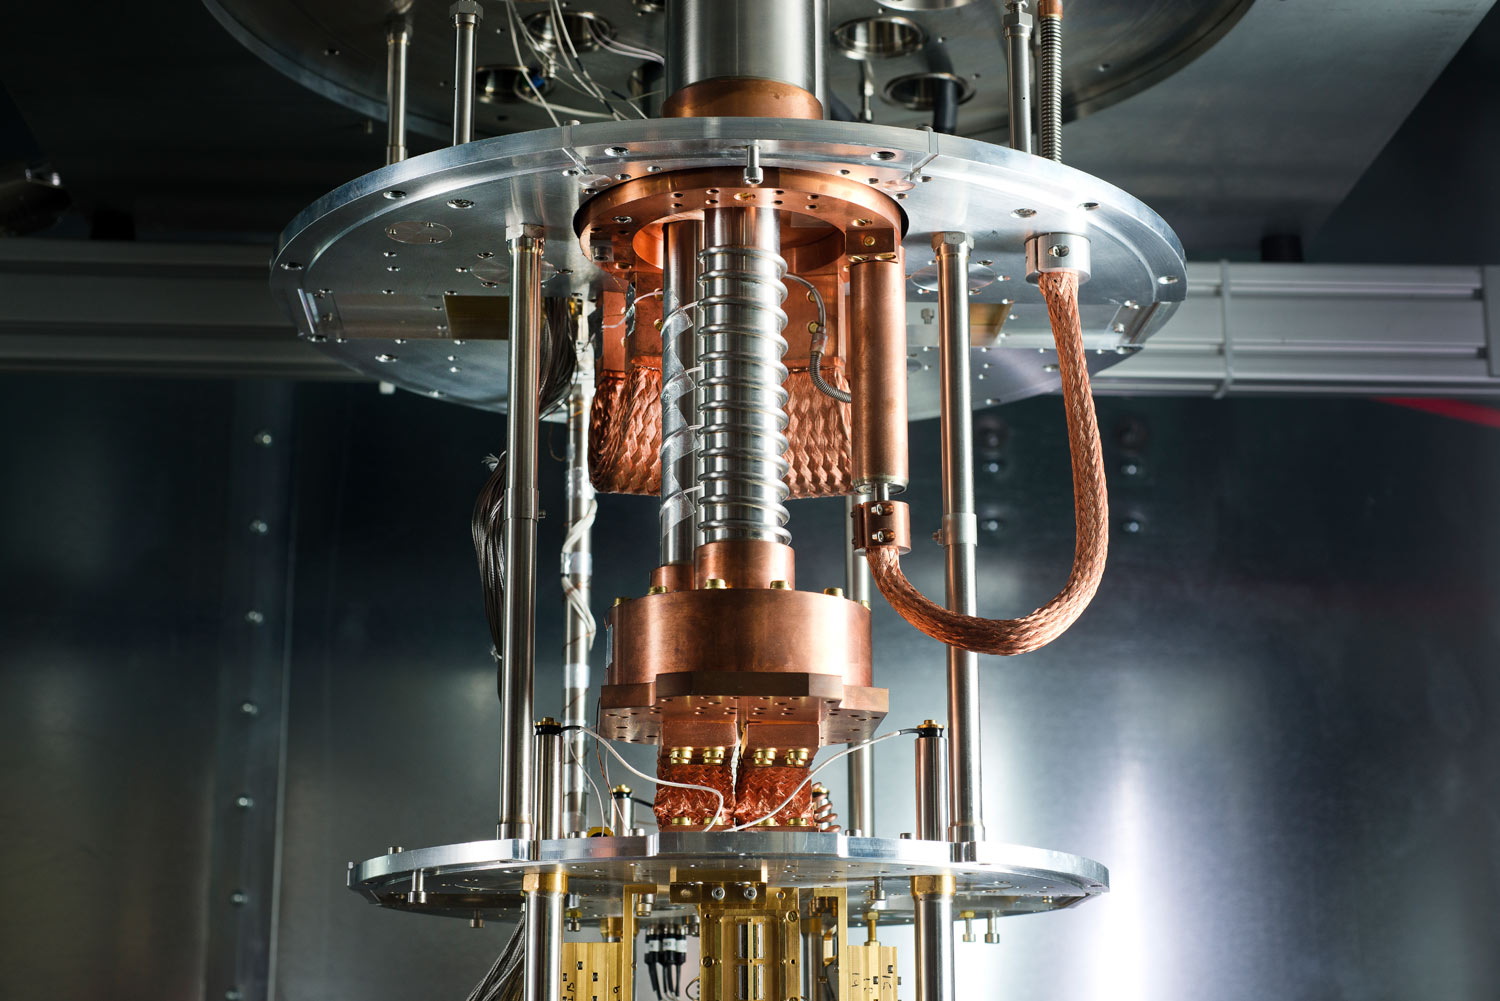
\includegraphics[trim=0 0 0 0mm, width=0.9\textwidth]{Images/cryostate.jpg}
		\end{column}
	\end{columns}
	\vspace*{0.5cm}
	\footnotesize\textcolor{tugreen}{$\blacktriangleright$}\,\,\cite{Inc.2016}\normalsize
\end{frame}}


\begin{center}
	\includeslide{dwave}
\end{center}

\noindent text


\mode<presentation>{\begin{frame}{Universal QC}\label{uniqc}
	\begin{columns}[T]
		\begin{column}{0.5\textwidth}
			\centering
			NMR \\
			\vspace{0.3cm}
			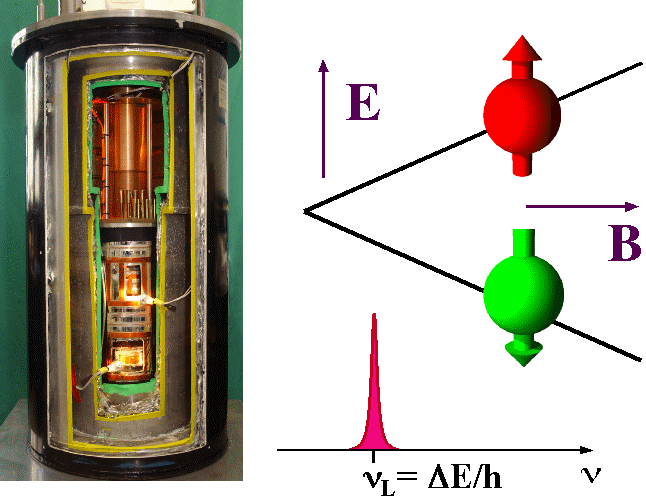
\includegraphics[trim=0 0 0 0mm, width=0.75\textwidth]{Images/nmr-e3} \\
			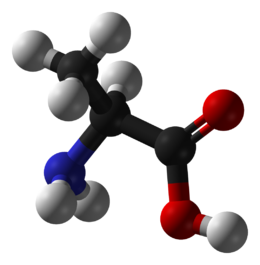
\includegraphics[trim=0 0 0 0mm, width=0.6\textwidth]{Images/nmr-alanine}
		\end{column}
		\begin{column}{0.5\textwidth}
			\centering
			\uncover<2->{Transmons \\
			\vspace{0.3cm}
    		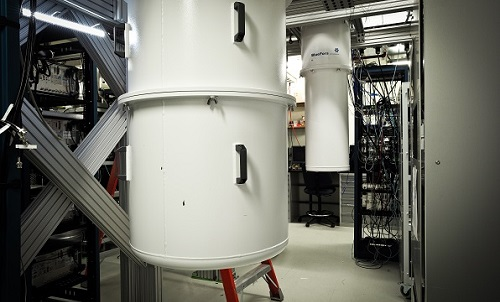
\includegraphics[trim=0 0 0 0mm, width=0.9\textwidth]{Images/ibm-cryo.jpg} \\
    		\vspace*{1.0cm}
    		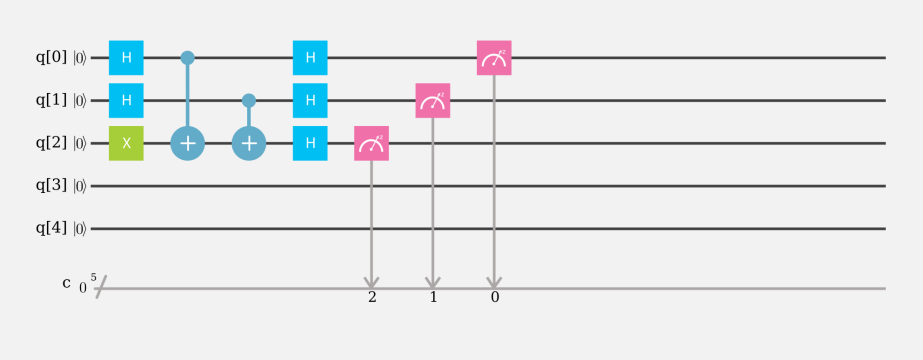
\includegraphics[trim=0 0 0 0mm, width=0.95\textwidth]{Images/ibm-composer} \\
    		Cloud-accessible!}
		\end{column}
	\end{columns}
	\vspace*{0.3cm}
	\footnotesize\textcolor{tugreen}{$\blacktriangleright$}\,\,\cite{Computing2017}\normalsize
\end{frame}}

\begin{center}
	\includeslide{uniqc}
\end{center}

\noindent text

\section{Spin Networks}

\subsection{Role in Quantum Computing}

\mode<presentation>{\begin{frame}[t]{QC Architecture}\label{architecture}
	\begin{columns}[T]
		\begin{column}{0.5\textwidth}
			\centering
   			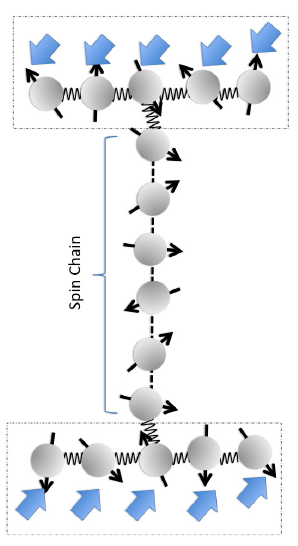
\includegraphics[trim=0mm 0 0 0mm, width=0.7\textwidth]{Images/processor}
		\end{column}
		\begin{column}{0.5\textwidth}
			\vspace*{1.0cm}
			\begin{itemize}
    			\item Distributed components
    			\item Smaller system size $\rightarrow$ less disturbance
    			\item Quantum wires without external control
    			\item Same material as processor
    		\end{itemize}
    		\vspace*{1.0cm}
    		$\rightarrow$ Spin Networks
		\end{column}
	\end{columns}
   	\footnotesize\textcolor{tugreen}{$\blacktriangleright$}\,\,\cite{Bose2014}\normalsize
\end{frame}}


\begin{center}
	\includeslide{architecture}
\end{center}

\noindent text


\mode<presentation>{\begin{frame}{Perfect State Transfer}\label{pst} %[fragile,t] for listings
	\begin{exampleblock}{}
	\setlength\abovedisplayskip{-8pt}
	\begin{center}
		\[H_{XX}=\frac{1}{2}J\sum_{i=1}^{N}{\left[\sigma_i^x\sigma_{i-1}^x + \sigma_i^y\sigma_{i-1}^y\right]}\]
	\end{center}
	\end{exampleblock} 
	Perfect State Transfer happens if
	\[ \mathfrak{F}(t) = \frac{\lvert f^N_{r,s}(t)\rvert\cos{\lambda}}{3} + \frac{\lvert f^N_{r,s}(t)\rvert^2}{6} + \frac{1}{2} = 1\]
	\vspace*{-0.7cm}
	\begin{exampleblock}{}
	\setlength\abovedisplayskip{-8pt}
	\begin{center}
		\[\lvert f^N_{r,s}(t)\rvert = \lvert \braket{r|\text{e}^{-iHt}|s}\rvert = 1\]
	\end{center}
	\end{exampleblock}
\end{frame}}

\begin{center}
	\includeslide{pst}
\end{center}

\noindent text


\mode<presentation>{\begin{frame}{Graphs}\label{graphs}
	\begin{exampleblock}{}
	\setlength\abovedisplayskip{-8pt}
	\begin{center}
		$G = (V,E)$
	\end{center}
	\end{exampleblock}
	Example: $V = \{1,2,3\}, E = \{\{1,2\},\{2,3\}\}$
	\begin{center}
		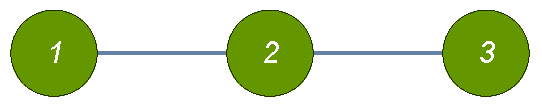
\includegraphics[trim=0mm 0 0 0mm, width=0.7\textwidth]{Images/chain3-graph}
	\end{center}
	Algebraic treatment through adjacency matrices:
	\begin{exampleblock}{}
	\setlength\abovedisplayskip{-8pt}
	\begin{center}
		$a_{ij} = \left\{
	\begin{array}{ll}
		1  & \{i,j\} \in E \\
		0  & \text{otherwise}
	\end{array}
\right.$	
	\end{center}
	\end{exampleblock}
\end{frame}}

\begin{center}
	\includeslide{graphs}
\end{center}

\noindent text


\mode<presentation>{\begin{frame}{Examples}\label{adjexamples}
	\begin{columns}[T]
		\begin{column}{0.5\textwidth}
			\centering
			\vspace{1.5cm}
   			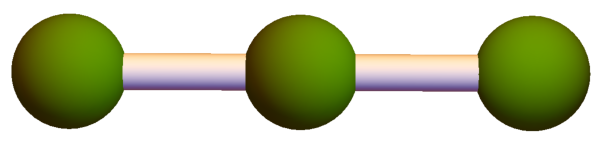
\includegraphics[trim=0mm 0 0 0mm, width=0.7\textwidth]{Images/chain3} \\
   			\vspace{1.0cm}
   			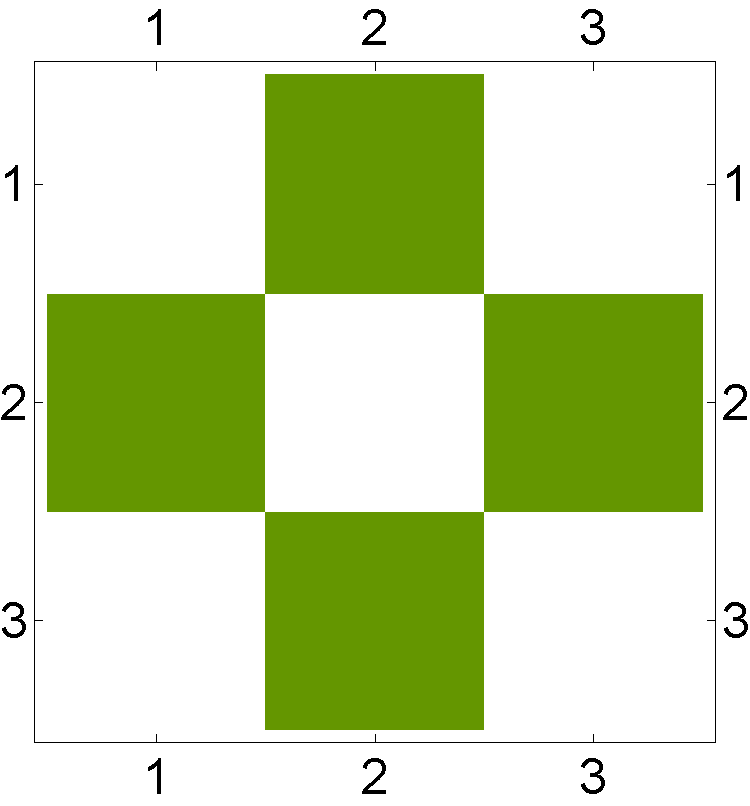
\includegraphics[trim=0mm 0 0 0mm, width=0.7\textwidth]{Images/chain3-adjmat}
		\end{column}
		\begin{column}{0.5\textwidth}
			\centering
   			\includegraphics[trim=0mm 0 0 0mm, width=0.6\textwidth]{Images/chain6vary-graph} \\
   			\includegraphics[trim=0mm 0 0 0mm, width=0.7\textwidth]{Images/chain6vary-adjmat}
		\end{column}
	\end{columns}
\end{frame}}

\begin{center}
	\includeslide{adjexamples}
\end{center}

\noindent text


\subsection{Perfect State Transfer}

\mode<presentation>{\begin{frame}{Identifying PST Graphs}\label{identifyPST}
	\begin{exampleblock}{}
	\setlength\abovedisplayskip{-8pt}
	\begin{center}
		$\text{e}^{-\text{i}H2t} \mbeq \text{1}$	
	\end{center}
	\end{exampleblock}
	\begin{itemize}
		\item Restrict $\mathcal{H}$ to single excitation space $\rightarrow$ adjacency matrix
		\item PST then means
			\begin{align*}
	\begin{pmatrix}
		1\\0\\0
	\end{pmatrix}
	\rightarrow
	\begin{pmatrix}
		0\\0\\1
	\end{pmatrix}
	\,\,\, \text{by} \,\,\,\, P_\pi = 
	\begin{pmatrix}
		0 & 0 & 1 \\
		0 & 1 & 0 \\
		1 & 0 & 0 \\
	\end{pmatrix}
			\end{align*}
		\item Check time evolution at half that time
	\end{itemize}
	\begin{exampleblock}{}
	\setlength\abovedisplayskip{-8pt}
	\begin{center}
		$\text{e}^{-\text{i}Ht} \mbeq P_\pi$	
	\end{center}
	\end{exampleblock}
\end{frame}}

\begin{center}
	\includeslide{identifyPST}
\end{center}

\noindent text


\mode<presentation>{\begin{frame}{Graph Product}\label{graphproduct}
	\begin{exampleblock}{}
	\setlength\abovedisplayskip{-8pt}
	\begin{center}
		$A_{G\times H} = A_G \otimes \text{1}_{\left|V_H\right|} + \text{1}_{\left|V_G\right|} \otimes A_H$
	\end{center}
	\end{exampleblock}
	\begin{columns}[T]
		\begin{column}{0.33\textwidth}
			\centering
   			\includegraphics[trim=0mm 0 0 0mm, width=1.0\textwidth]{Images/graphprod_chain3_square} \\
		\end{column}
		\begin{column}{0.33\textwidth}
			\centering
   			\includegraphics[trim=0mm 0 0 0mm, width=1.0\textwidth]{Images/graphprod_chain3_chain2_square} \\
		\end{column}
		\begin{column}{0.33\textwidth}
			\centering
   			\includegraphics[trim=0mm 0 0 0mm, width=1.0\textwidth]{Images/graphprod_switch_square.pdf} \\
		\end{column}
	\end{columns}
\end{frame}}

\begin{center}
	\includeslide{graphproduct}
\end{center}

\noindent text


\mode<presentation>{\begin{frame}{Graph Product}\label{graphproductfidelity}
	\begin{exampleblock}{}
	\setlength\abovedisplayskip{-8pt}
	\begin{center}
		$ f^{\left|V_{G\times H}\right|}_{(r,r'),(s,s')}(t) = f^{\left|V_G\right|}_{r,s}(t)\cdot f^{\left|V_H\right|}_{r',s'}(t) $
	\end{center}
	\end{exampleblock}
	\vspace*{-0.5cm}
	\begin{align*}
		\left|f^{\left|V_G\right|}_{r,s}(t)\right| &= 1 \text{ for } t = \tau_G \\ 
		\left|f^{\left|V_H\right|}_{r',s'}(t)\right| &= 1 \text{ for } t = \tau_H \\ 
		\left|f^{\left|V_{G\times H}\right|}_{(r,r'),(s,s')}(t)\right| &= 1 \text{ for } t = \tau_{G\times H}
	\end{align*}
	\vspace*{-1.0cm}
	\begin{exampleblock}{}
	\setlength\abovedisplayskip{-8pt}
	\begin{center}
		$ \text{iff }\frac{\tau_G}{\tau_H} \in \mathbb{Q}$
	\end{center}
	\end{exampleblock}
\end{frame}}

\begin{center}
	\includeslide{graphproductfidelity}
\end{center}

\noindent text


\subsection{Quantum Routing}

\mode<presentation>{\begin{frame}{Quantum Routing}\label{routing}
	\begin{exampleblock}{}
	\setlength\abovedisplayskip{-8pt}
	\begin{center}
		\[ H = \frac{1}{2}J\sum_{i=2}^{N}\left[\sigma_1^x\sigma_i^x + \sigma_1^y\sigma_i^y\right] + \sum_{i=1}^{N}h_i\sigma_i^z \]
	\end{center}
	\end{exampleblock}
	\begin{columns}[T]
		\begin{column}{0.5\textwidth}
		\begin{center}
			\includegraphics[trim=0mm 0 0 10mm, width=0.9\textwidth]{Images/switch_selfloops}
		\end{center}
		\end{column}
		\begin{column}{0.5\textwidth}
		\vspace{1.0cm}
		\begin{itemize}
			\item Local magnetic fields
			\item Diagonal entries in adjacency matrix
			\item Global offset field allows switching
		\end{itemize}
		\end{column}
	\end{columns}
\end{frame}}

\begin{center}
	\includeslide{routing}
\end{center}

\noindent text


\mode<presentation>{\begin{frame}{Quantum Routing}\label{routing1}
	\begin{columns}[T]
		\begin{column}{0.5\textwidth}
		\begin{center}
			\includegraphics[trim=0mm 0 0 10mm, width=0.65\textwidth]{Images/switch_selfloops} \\
			\vspace{0.5cm}
			\includegraphics[trim=0mm 0 0 10mm, width=0.7\textwidth]{Images/switch-permutation}
		\end{center}
		\end{column}
		\begin{column}{0.5\textwidth}
		\begin{center}
			\includegraphics[trim=0mm 0 0 10mm, width=0.5\textwidth]{Images/switch_square.png} \\
			\vspace{0.4cm}
			\includegraphics[trim=0mm 0 0 10mm, width=0.8\textwidth]{Images/switchsquare-permutation}
		\end{center}
		\end{column}
	\end{columns}
\end{frame}}

\begin{center}
	\includeslide{routing1}
\end{center}

\noindent text


\mode<presentation>{\begin{frame}{Quantum Routing}\label{routing2}
	\begin{columns}[T]
		\begin{column}{0.5\textwidth}
		\begin{center}
			\includegraphics[trim=0mm 0 0 10mm, width=0.65\textwidth]{Images/switch_selfloops} \\
			\vspace{0.5cm}
			\includegraphics[trim=0mm 0 0 10mm, width=0.7\textwidth]{Images/switch2-permutation}
		\end{center}
		\end{column}
		\begin{column}{0.5\textwidth}
		\begin{center}
			\includegraphics[trim=0mm 0 0 10mm, width=0.5\textwidth]{Images/switch_square.png} \\
			\vspace{0.4cm}
			\includegraphics[trim=0mm 0 0 10mm, width=0.8\textwidth]{Images/switchsquare2-permutation}
		\end{center}
		\end{column}
	\end{columns}
\end{frame}}

\begin{center}
	\includeslide{routing2}
\end{center}

\noindent text


\subsection{Designing Networks}

\mode<presentation>{\begin{frame}{Higher Excitation Spaces}\label{hes}
	\begin{columns}[T]
		\begin{column}{0.5\textwidth}
		\begin{center}
			\includegraphics[trim=0mm 0 0 0mm, width=1.0\textwidth]{Images/method4-solution-chain2square} \\
			\includegraphics[trim=0mm 0 0 0mm, width=0.7\textwidth]{Images/chain2square-hes2-pst-marked}
		\end{center}
		\end{column}
		\begin{column}{0.5\textwidth}
		\begin{center}
			\includegraphics[trim=0mm 0 0 0mm, width=0.6\textwidth]{Images/chain2-cube} \\
			\includegraphics[trim=0mm 0 0 0mm, width=0.7\textwidth]{Images/chain2cube-hes2}
		\end{center}
		\end{column}
	\end{columns}
\end{frame}}

\begin{center}
	\includeslide{hes}
\end{center}

\noindent text


\mode<presentation>{\begin{frame}{Renormalization}\label{renormalization}
	\begin{columns}[T]
		\begin{column}{0.5\textwidth}
		\begin{center}
			\includegraphics[trim=0mm 0 0 0mm, width=1.0\textwidth]{Images/chain2-hypercube}
		\end{center}
		\end{column}
		\begin{column}{0.5\textwidth}
		\begin{center}
			\includegraphics[trim=0mm 0 0 0mm, width=0.85\textwidth]{Images/hypercube-to-perfect-couplings}
		\end{center}
		\end{column}
	\end{columns}
	\footnotesize\textcolor{tugreen}{$\blacktriangleright$}\,\,\cite{Christandl2005}\normalsize
\end{frame}}

\begin{center}
	\includeslide{renormalization}
\end{center}

\noindent text


\mode<presentation>{\begin{frame}{Renormalization}\label{renormalization2}	
	\begin{columns}[T]
		\begin{column}{0.5\textwidth}
		\begin{center}
			\includegraphics[trim=0mm 0 0 0mm, width=0.8\textwidth]{Images/eg-renorm-3}
		\end{center}
		\end{column}
		\begin{column}{0.5\textwidth}
		\begin{center}
			\includegraphics[trim=0mm 0 0 0mm, width=0.5\textwidth]{Images/eg-triplearmstar-uniform} \\
			\vspace*{0.3cm}
			\includegraphics[trim=0mm 0 0 0mm, width=0.45\textwidth]{Images/chain2square-hes2-pst-marked} \\
			\vspace*{0.3cm}
			\includegraphics[trim=0mm 0 0 0mm, width=0.5\textwidth]{Images/eg-pentaarmstar-uniform}
		\end{center}
		\end{column}
	\end{columns}
\end{frame}}

\begin{center}
	\includeslide{renormalization2}
\end{center}

\noindent text


\mode<presentation>{\begin{frame}{Network Construction}\label{method}
	\begin{columns}[T]
		\begin{column}{0.5\textwidth}
		\begin{center}
			\includegraphics[trim=0mm 0 0 0mm, width=0.65\textwidth]{Images/method7-graph}
		\end{center}
		\begin{align*}
	\begin{pmatrix}
		y_1 & y_2 & y_3 \\
		z_1 & z_2 & z_3 
	\end{pmatrix}
	\cdot
	\begin{pmatrix}
		a_1 & b_1 \\
		a_2 & b_2 \\
		a_3 & b_3 
	\end{pmatrix}
	\cdot
	\begin{pmatrix}
		1 \\
		0
	\end{pmatrix}
	&\mbeq
	\begin{pmatrix}
		1 \\
		0
	\end{pmatrix}
\end{align*}
		\end{column}
		\begin{column}{0.5\textwidth}
		\begin{center}
			\uncover<2->{\includegraphics[trim=0mm 0 0 0mm, width=0.5\textwidth]{Images/method7-solution-2chain3} \\
			\vspace*{0.8cm}
			\includegraphics[trim=0mm 0 0 0mm, width=0.45\textwidth]{Images/method7-solution-chain2square-hes2}}
			%\vspace*{0.3cm}
			%\includegraphics[trim=0mm 0 0 0mm, width=0.5\textwidth]{Images/eg-pentaarmstar-uniform}
		\end{center}
		\end{column}
	\end{columns}

\end{frame}}

\begin{center}
	\includeslide{method}
\end{center}

\noindent text


\mode<presentation>{\begin{frame}{Conclusion}\label{conclusion}
	\begin{itemize}
		\item Exponential speedup for some problems
		\item Some classical algorithms may be impossible to implement on QC
		\item Designing networks for defined system topologies is possible 
		\item Realization of most networks questionable		
	\end{itemize}
\end{frame}}

\begin{center}
	\includeslide{conclusion}
\end{center}

\noindent text


\end{document}
